\documentclass[10pt,a4paper,fleqn]{article}
%%%%%%%%%%%%%%%%%%%%%%%%%%%%%%%%%%%%%%%%%%%%%%%%%%%
%% Load Packages
%%%%%%%%%%%%%%%%%%%%%%%%%%%%%%%%%%%%%%%%%%%%%%%%%%%

% Math
\usepackage{algorithm}
\usepackage{algcompatible}
\usepackage{algpseudocode}
\usepackage{amsmath}	% package to display formulas, provided by the American Mathematical Society 
\usepackage{amssymb}  
%\usepackage{siunitx}	% package to use SI units
\usepackage{nicefrac}	% allows writing fracs as a/b
\usepackage{mathtools}	% left indices
\usepackage{units}
\usepackage{cancel}
\usepackage{mathtools}

% Graphics
\usepackage{graphicx}	% package to inlcude eps grahics

\usepackage{pgf}		% package to generate graphics in Latex, provides the pgfpicture enviroment
\usepackage{tikz}		% frontend for pgf
\usepackage{pgfplots}	% package to generate 2D/3D plots, bases on tikz, documentation on http://pgfplots.sourceforge.net/pgfplots.pdf
\usepackage{tikz-3dplot}
%\pgfplotsset{compat=1.6}
\usepackage{psfrag}		% load eps, and write text into it

% Misc
\usepackage{fancyhdr}
\setcounter{MaxMatrixCols}{12}
\usepackage{hyperref}
\usepackage[margin=3.0cm]{geometry}
\usepackage[toc,page]{appendix}
\usepackage{siunitx}


\usepackage{booktabs}

\usepackage{listings}
\usepackage{mathtools}
\usepackage{multirow}
\usepackage{relsize}

\usepackage[font+=small]{caption}
\usepackage[font+=small]{subcaption}
\captionsetup{subrefformat=parens}

\usepackage{siunitx}
\sisetup{group-separator = {,}, group-minimum-digits=3}
\sisetup{range-phrase=--}
\sisetup{range-units=single}

\usepackage{url}
%%%%%%%%%%%%%%%%%%%%%%%%%%%%%%%%%%%%%%%%%%%%%%%%%%%
%% pgfplot settings
%%%%%%%%%%%%%%%%%%%%%%%%%%%%%%%%%%%%%%%%%%%%%%%%%%%

%\pgfplotsset{compat=1.6}	% Pgfplot compatibility mode 1.6

%%%%%%%%%%%%%%%%%%%%%%%%%%%%%%%%%%%%%%%%%%%%%%%%%%%
%% Tikz general settings
%%%%%%%%%%%%%%%%%%%%%%%%%%%%%%%%%%%%%%%%%%%%%%%%%%%
%%% use the tikz calc lib for the bounding box
\usetikzlibrary{calc}

%%%%%%%%%%%%%%%%%%%%%%%%%%%%%%%%%%%%%%%%%%%%%%%%%%%
%% Misc
%%%%%%%%%%%%%%%%%%%%%%%%%%%%%%%%%%%%%%%%%%%%%%%%%%%
\usepackage{fancyhdr}
\graphicspath{{img//}}

%%%%%%%%%%%%%%%%%%%%%%%%%%%%%%%%%%%%%%%%%%%%%%%%%%%
%% My commands
%%%%%%%%%%%%%%%%%%%%%%%%%%%%%%%%%%%%%%%%%%%%%%%%%%%
\def\highdot{\!\raisebox{.5em}{$\cdot$}}

\newcommand{\ssin}[0]{\operatorname{s}}
\newcommand{\scos}[0]{\operatorname{c}}
\newcommand{\stan}[0]{\operatorname{t}}
\newcommand{\atantwo}[0]{\operatorname{atan2}}
\newcommand{\asin}[0]{\operatorname{asin}}
\DeclareMathOperator\sign{sign}

%%%%%%%%%%%%%%%%%%%%%%%%%%%%%%%%%%%%%%%%%%%%%%%%%%%
%% My symbols
%%%%%%%%%%%%%%%%%%%%%%%%%%%%%%%%%%%%%%%%%%%%%%%%%%%
\newcommand{\pos}[0]{\bVec{p}} % position
\newcommand{\vel}[0]{\bVec{v}} % velocity
\newcommand{\acc}[0]{\bVec{a}} % acceleration
\newcommand{\jerk}[0]{\bVec{j}} % jerk
\newcommand{\snap}[0]{\bVec{s}} % snap

\newcommand{\quatrot}[0]{\boldsymbol{\Lambda}}

\newcommand{\qx}[0]{\ensuremath{q_x}}
\newcommand{\qy}[0]{\ensuremath{q_y}}
\newcommand{\qz}[0]{\ensuremath{q_z}}
\newcommand{\qw}[0]{\ensuremath{q_w}}

%%%%%%%%%%%%%%%%%%%%%%%%%%%%%%%%%%%%%%%%%%%%%%%%%%%%%%%%%%%%%%%%%%%%%%%%%%%%%%%%
% Definitions
\newcommand{\bVec}[1]{\mathbf{#1}}
\newcommand{\sVec}[1]{\begin{bmatrix} #1 \end{bmatrix}}
\newcommand{\norm}[1]{\left\lVert#1\right\rVert}
\newcommand{\abs}[1]{\left\lvert#1\right\rvert}
\newcommand{\diag}[1]{\operatorname{diag}\left(#1 \right) }

\newcommand{\vect}[3]{{_{\mathsmaller{\mathrm{#2}}}\mathbf{#1}_{\mathsmaller{\mathrm{#3}}}}} % vector: _{#2}_{#1}_{#3}
\newcommand{\vectss}[4]{{_{\mathsmaller{\mathrm{#2}}}\mathbf{#1}_{\mathsmaller{\mathrm{#3}}}^{\mathsmaller{\mathrm{#4}}}}} % vector with superscript
%\newcommand{\vecttrans}[3]{\vectss{#1}{#2}{#3}{T}} % transposed vector: _{#2}_{#1}_{#3}^T
\newcommand{\vecttrans}[3]{{_{\mathsmaller{\mathrm{#2}}}\mathbf{#1}_{\mathsmaller{\mathrm{#3}}}^{\mathsmaller{\top}}}} % transposed vector: _{#2}_{#1}_{#3}^T
\newcommand{\vectbar}[3]{{_{\mathsmaller{\mathrm{#2}}}\bar{\mathbf{#1}}_{\mathsmaller{\mathrm{#3}}}}} % differentiated vector: _{#2}_{#1}_{#3}
\newcommand{\vectdot}[3]{{_{\mathsmaller{\mathrm{#2}}}\dot{\mathbf{#1}}_{\mathsmaller{\mathrm{#3}}}}} % differentiated vector: _{#2}_{#1}_{#3}
\newcommand{\vectddot}[3]{{_{\mathsmaller{\mathrm{#2}}}\ddot{\mathbf{#1}}_{\mathsmaller{\mathrm{#3}}}}} % differentiated vector: _{#2}_{#1}_{#3}
\newcommand{\vectdddot}[3]{{_{\mathsmaller{\mathrm{#2}}}\dddot{\mathbf{#1}}_{\mathsmaller{\mathrm{#3}}}}} % differentiated vector: _{#2}_{#1}_{#3}

%%%%%%%%%%%%%%%%%%%%%%%%%%%%%%%%%%%%%%%%%%%%%%%%%%%%%%%%%%%%%%%%%%%%%%%%%%%%%%%%
% Symbols

\newcommand{\wfr}[0]{\ensuremath{W}} % world frame
\newcommand{\bfr}[0]{\ensuremath{B}} % body frame
\newcommand{\cfr}[0]{\ensuremath{C}} % C-frame

\newcommand{\gravacc}[0]{\ensuremath{g}} % gravitational acceleration
\newcommand{\gravityvec}[0]{\bVec{\gravacc}} % gravity vector

\newcommand{\ori}[1]{\bVec{R}_{\!\mathsmaller{\mathrm{#1}}}} % orientation
\newcommand{\heading}[0]{\psi} % heading or yaw angle

\newcommand{\bodyrate}[0]{\omega} % component of body rates vector
\newcommand{\bodyrates}[0]{\boldsymbol{\bodyrate}} % body rates vector

\newcommand{\torqueinput}[0]{\tau} % component of torque input vector
\newcommand{\torqueinputs}[0]{\boldsymbol{\tau}} % torque input vector
\newcommand{\inertia}[0]{\bVec{J}} % inertia matrix
\newcommand{\gyrotorques}[0]{\vect{\torqueinputs}{}{g}} % torques from propeller gyro effects
\newcommand{\bodytorque}[0]{\eta}
\newcommand{\bodytorques}[0]{\boldsymbol{\bodytorque}}
\newcommand{\thrust}[0]{c} % mass normalized thrust
\newcommand{\horzthrustcoeff}[0]{k_h} % thrust change coefficient wrt to body horizontal velocity
\newcommand{\rotthrust}[1]{f_{#1}}
\newcommand{\armlength}[0]{l}
\newcommand{\torquecoeff}[1]{\kappa_{#1}}
\newcommand{\mass}[0]{m}
\newcommand{\rottorque}[1]{\tau_{#1}}
\newcommand{\motinput}[1]{u_{#1}}
\newcommand{\mapcoeff}[2]{k_{#2}^{#1}}
\newcommand{\motdyn}[0]{\alpha_{\mathsmaller{\mathrm{mot}}}}

\newcommand{\klqr}[0]{\ensuremath{\bVec{K}_{lqr}}}
\newcommand{\lqrstate}[0]{\ensuremath{\bVec{s}}}
\newcommand{\lqrinput}[0]{\ensuremath{\bVec{u}}}

\newcommand{\dragcoeff}[1]{\ensuremath{d}_{\!\mathsmaller{\mathrm{#1}}}} % rotor drag coefficient
\newcommand{\dragmat}[0]{\bVec{D}} % rotor drag matrix
\newcommand{\amat}[0]{\bVec{A}} % 
\newcommand{\bmat}[0]{\bVec{B}} % 

\newcommand{\yawRef}[0]{\heading_{\mathsmaller{\mathrm{ref}}}} % 
\newcommand{\uvec}[0]{\bVec{e}} % symbol for unit vector

% Title page
\title{Theory and Math Behind RPG Quadrotor Control}

\author{
  Matthias Faessler and Flavio Fontana
}

\date{\today}


% Begin document________________________________________________________________
\begin{document}

\pagestyle{fancy}             % Fancy headings
\pagenumbering{arabic}				% Begin arabic page numbering (1,2,...)

\maketitle
\tableofcontents
\newpage


\section{Introduction}

\begin{figure}[t]
   \centering
   \includegraphics[width=0.8\textwidth]{img/quad_picture.pdf}
   \caption{First-person-view racing inspired quadrotor platform used for the experiments presented in~\cite{Faessler18ral}.}
   \label{fig:quad_picture}
\end{figure}

In this document, we summarized the theory and math behind the quadrotor control algorithms developed at the \emph{Robotics and Perception Group} as they are implemented in our \href{https://github.com/uzh-rpg/rpg_quadrotor_control}{rpg\_quadrotor\_control} repository.
If you spot any typos or mistakes or want to improve or add something, please open an issue or send us a pull request on \url{https://github.com/uzh-rpg/rpg_quadrotor_control}.
The control algorithms presented here are published in~\cite{Faessler18ral}, for which we developed the quadrotor shown in Fig.~\ref{fig:quad_picture}, and in~\cite{Faessler17ral}.

\section{Nomenclature} \label{sec:nomenclature}

\begin{figure}[h]
   \centering
   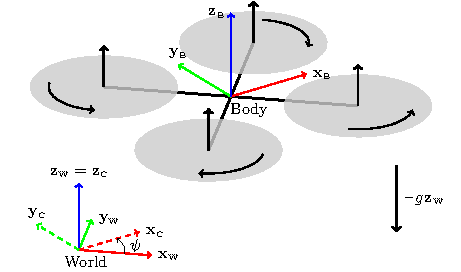
\includegraphics[width=0.8\textwidth]{img/quadrotor.pdf}
   \caption{Schematics of the considered quadrotor model with the used coordinate systems and rotor forces.}
   \label{fig:quad}
\end{figure}

In this work, we make use of a world frame $\wfr$ with orthonormal basis ${\left\{ \vect{x}{}{\wfr}, \vect{y}{}{\wfr}, \vect{z}{}{\wfr} \right\}}$ represented in world coordinates and a body frame $\bfr$ with orthonormal basis ${\left\{ \vect{x}{}{\bfr}, \vect{y}{}{\bfr}, \vect{z}{}{\bfr} \right\}}$ also represented in world coordinates.
The body frame is fixed to the quadrotor with an origin coinciding with its center of mass as depicted in Fig.~\ref{fig:quad}.
The rotor numbering and rotation directions can also be seen in Fig.~\ref{fig:quad}.
The quadrotor is subject to a gravitational acceleration $\gravacc$ in negative $\vect{z}{}{\wfr}$ direction.
We denote the position of the quadrotor's center of mass as $\pos$, and its derivatives, velocity, acceleration, jerk, and snap as $\vel$, $\acc$, $\jerk$, and $\snap$, respectively.
We represent the quadrotor's orientation as a rotation matrix ${\ori{} = \sVec{\vect{x}{}{\bfr} & \vect{y}{}{\bfr} & \vect{z}{}{\bfr}}}$ and its body rates (i.e., the angular velocity) as $\bodyrates$ represented in body coordinates.
Finally, we denote quantities that can be computed from a reference trajectory as \emph{reference values} and quantities that are computed by an outer loop feedback control law and passed to an inner loop controller as \emph{desired values}.
A reference trajectory consists of the reference position $\vect{\pos}{}{ref}$, the reference velocity $\vect{\vel}{}{ref}$, the reference acceleration $\vect{\acc}{}{ref}$, the reference jerk $\vect{\jerk}{}{ref}$, and the reference snap $\vect{\snap}{}{ref}$, as well as a reference heading $\heading_{\mathsmaller{\mathrm{ref}}}$, a reference heading rate $\dot{\heading}_{\mathsmaller{\mathrm{ref}}}$, and a reference heading acceleration $\ddot{\heading}_{\mathsmaller{\mathrm{ref}}}$.

\section{Dynamical Model} \label{sec:dynamical_model}

We consider a quadrotor that is modeled as a rigid body which is controlled by four single rotor thrusts $\rotthrust{i}$ as illustrated in Fig.~\ref{fig:quad}.
By changing these four single rotor thrusts, a three axis torque $\bodytorques$ and a mass normalized collective thrust $\thrust$ can be applied on the quadrotor's body.
The relation of the single rotor thrusts to the collective thrust and the body torques can be formulated using the coordinate system of Fig.~\ref{fig:quad} as
%
\begin{align}
	\bodytorques &= \begin{bmatrix} \frac{\sqrt{2}}{2}\armlength(\rotthrust{1} - \rotthrust{2} - \rotthrust{3} + \rotthrust{4}) \\
							\frac{\sqrt{2}}{2}\armlength(-\rotthrust{1} - \rotthrust{2} + \rotthrust{3} + \rotthrust{4}) \\
							\torquecoeff{1}\rotthrust{1} - \torquecoeff{2}\rotthrust{2} + \torquecoeff{3}\rotthrust{3} - \torquecoeff{4}\rotthrust{4}
						\end{bmatrix}, \label{eq:torque_mixing}\\
    \mass \thrust &= \rotthrust{1} + \rotthrust{2} + \rotthrust{3} + \rotthrust{4}, \label{eq:collective_thrust_mixing}
\end{align}
%
where $\armlength$ is the quadrotor's arm length, ${\torquecoeff{i} = \torquecoeff{}(\rotthrust{i})}$ is a coefficient relating the drag torque and the thrust of a single rotor, and $\mass$ is the quadrotor's mass.
Note that unlike in~\cite{Lupashin14mech} and~\cite{Faessler16jfr}, we consider the rotor drag torque coefficient $\torquecoeff{}$ to be a function of the rotor thrust (cf. Fig~\ref{fig:kappa_load_cell}) and \emph{not a constant}.

We model the single rotor thrust $\rotthrust{}$ and drag torque $\rottorque{}$ as quadratic polynomials of the motor input $\motinput{}$ as
%
\begin{align}
	\rotthrust{}(\motinput{}) &= \mapcoeff{\rotthrust{}}{2} \motinput{}^2 + \mapcoeff{\rotthrust{}}{1} \motinput{} + \mapcoeff{\rotthrust{}}{0}, \label{eq:thrust_mapping}\\
	\rottorque{}(\motinput{}) &= \mapcoeff{\rottorque{}}{2} \motinput{}^2 + \mapcoeff{\rottorque{}}{1} \motinput{} + \mapcoeff{\rottorque{}}{0}, \label{eq:torque_mapping}
\end{align}
%
where the coefficients $\mapcoeff{\rotthrust{}}{j}$ and $\mapcoeff{\rottorque{}}{j}$ are identified by running a single motor with a propeller on a load cell and measuring the resulting forces and moments.
The motor input $\motinput{}$ corresponds to the command we can send to our electronic speed controllers in the range $[-1, \; 1]$.
We chose to have three coefficients since it approximates the measured values better than modeling the rotor thrust and drag torque with only a quadratic term, as proposed in e.g.~\cite{Michael10ram}. 
Fig.~\ref{fig:thrust_mapping_fit} compares the two methods for fitting the thrust mapping.
%
\begin{figure}[t]
   \centering
   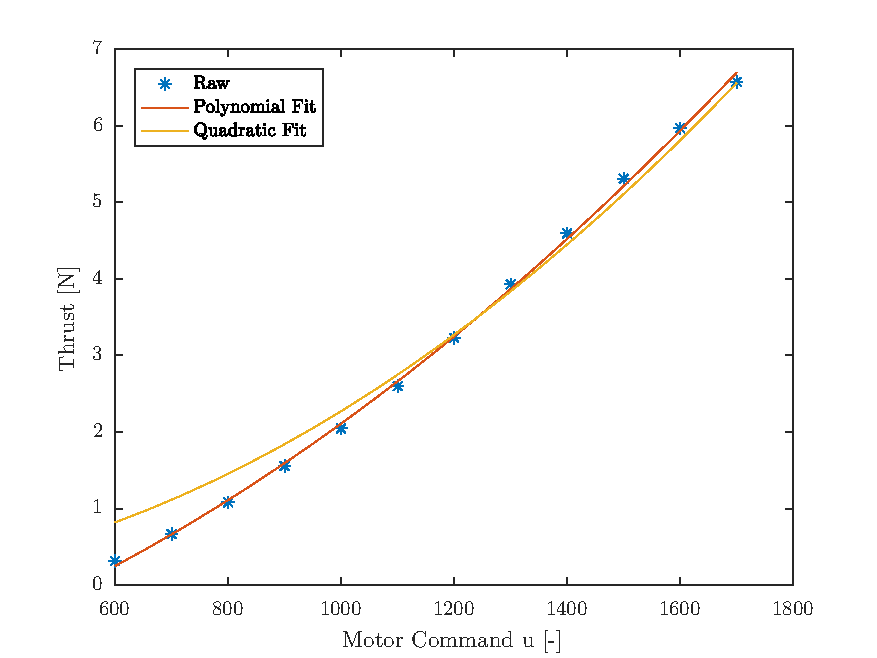
\includegraphics[width=0.8\textwidth]{img/thrust_mapping_fit_fpv.pdf}
   \caption{To approximate the thrust mapping for a single motor with propeller, we fit a second order polynomial into raw thrust measurements obtained by running the motor on a load cell. The polynomial fit approximates the measurements much better than a purely quadratic fit of the form $\rotthrust{}(\motinput{}) = \mapcoeff{\rotthrust{}}{2} \motinput{}^2$. Data is captured with stiff 6x4.5 inch propellers, Cobra CM-2208/20 2000Kv motors, and DYS XSD20A electronic speed controllers which are commanded through the Dshot300 protocol (Setup shown in Fig.~\ref{fig:quad_picture}).}
   \label{fig:thrust_mapping_fit}
\end{figure}
%
From~\eqref{eq:thrust_mapping} and~\eqref{eq:torque_mapping}, we can compute the rotor drag torque coefficient as
%
\begin{equation}
	 \torquecoeff{}(\rotthrust{}) = \frac{\rottorque{} \left( u = \frac{-\mapcoeff{\rotthrust{}}{1} + \sqrt{\left( \mapcoeff{\rotthrust{}}{1} \right)^2 - 4 \mapcoeff{\rotthrust{}}{2} \left( \mapcoeff{\rotthrust{}}{0} - \rotthrust{} \right)}}{2 \mapcoeff{\rotthrust{}}{2}} \right)}{\rotthrust{}}. 
	 \label{eq:rotor_drag_torque_coeff}
\end{equation}
%
Fig.~\ref{fig:kappa_load_cell} shows the identified values for the rotor drag torque coefficient and how it varies by about \SI{10}{\percent} over the entire range of available motor inputs.
%
\begin{figure}[t]
   \centering
   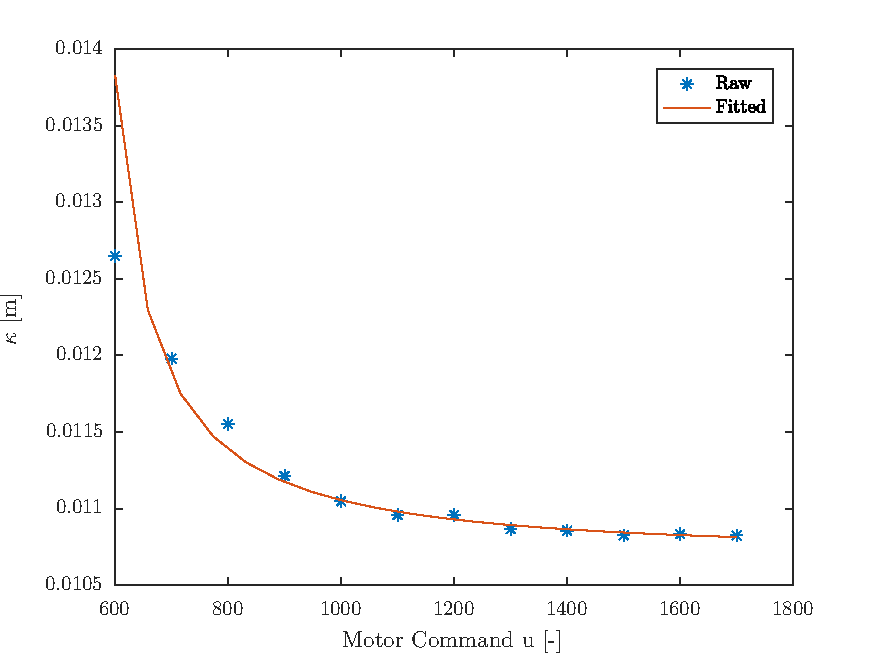
\includegraphics[width=0.8\textwidth]{img/kappa_load_cell_fpv.pdf}
   \caption{Values for $\torquecoeff{}$ estimated from load cell data obtained by dividing drag torque and thrust values for a motor and propeller. The fitted curve is the ratio of the fitted quadratic functions for measured thrust and drag torque in~\eqref{eq:thrust_mapping} and~\eqref{eq:torque_mapping}. Data is captured with stiff 6x4.5 inch propellers, Cobra CM-2208/20 2000Kv motors, and DYS XSD20A electronic speed controllers which are commanded through the Dshot300 protocol (Setup shown in Fig.~\ref{fig:quad_picture}).}
   \label{fig:kappa_load_cell}
\end{figure}
%
We consider the dynamical model of a quadrotor with rotor drag developed in~\cite{Kai17ifac} with no wind, stiff propellers, and no dependence of the rotor drag on the thrust.
Additionally, as in~\cite{Faessler17ral}, we model the dynamics of the single rotor thrusts as first order systems
%
\begin{equation}
	\dot{\rotthrust{}} = \frac{1}{\motdyn} \left( \rotthrust{des} - \rotthrust{} \right)
		\label{eq:motor_dynamics}
\end{equation}
%
where the time constant $\motdyn$ is identified from applying step inputs to a single motor with propeller on a load cell as illustrated in Fig.~\ref{fig:thrust_transients}.
%
\begin{figure}[t]
   \centering
   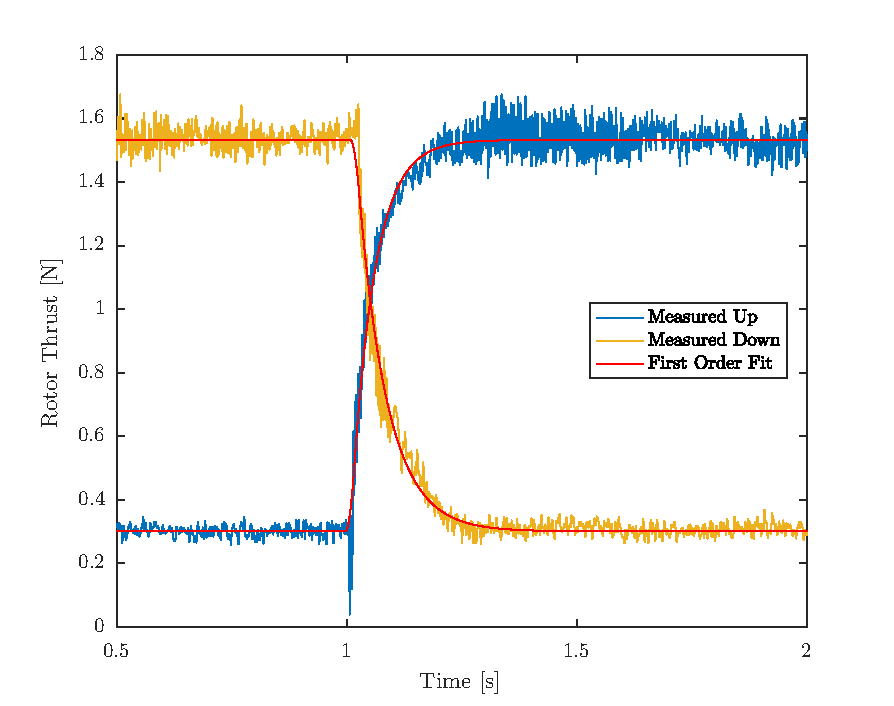
\includegraphics[width=0.8\textwidth]{img/thrust_transient.pdf}
   \caption{Thrust transients of a single motor with propeller on a load cell for a step up (blue) and a step down (red). A first order system fit for both is overlaid in red. Data is captured with stiff 6x4.5 inch propellers, Cobra CM-2208/20 2000Kv motors, and DYS XSD20A electronic speed controllers which are commanded through the Dshot300 protocol (Setup shown in Fig.~\ref{fig:quad_picture}).}
   \label{fig:thrust_transients}
\end{figure}
%
From these load-cell experiments we found that for modern ESCs that actively break the motor when spinning down, the time constant is almost identical when spinning a motor up or down and we therefore do not need to separate those cases.
Because of that, also the bod torques have first order dynamics with the same time constant as the single rotor thrusts.
According to these models in~\cite{Kai17ifac} and~\cite{Faessler17ral}, the dynamics of the position $\pos$, velocity $\vel$, orientation $\ori{}$, body rates $\bodyrates$, and body torques $\bodytorques$ can be written as
%
\begin{align}
	\dot{\pos} &= \vel \label{eq:position_dynamics} \\
	\dot{\vel} &= - \gravacc \vect{z}{}{\wfr} + \thrust \vect{z}{}{\bfr} - \ori{} \dragmat \vecttrans{\ori{}}{}{} \vel \label{eq:velocity_dynamics} \\
	\dot{\ori{}} &= \ori{} \hat{\bodyrates} \label{eq:orientation_dynamics} \\
	\dot{\bodyrates} &= \inertia^{-1} \left( \bodytorques - \bodyrates \times \inertia \bodyrates - \gyrotorques - \amat \vecttrans{\ori{}}{}{} \vel - \bmat \bodyrates \right) \label{eq:body_rate_dynamics} \\
	\dot{\bodytorques} &= \frac{1}{\motdyn} \left( \vect{\bodytorques}{}{des} - \bodytorques \right)
	\label{eq:body_torque_dynamics}
\end{align}
%
where $\thrust$ is the mass-normalized collective thrust, ${\dragmat = \diag{\dragcoeff{x}, \dragcoeff{y}, \dragcoeff{z}}}$ is a constant diagonal matrix formed by the rotor-drag coefficients, $\hat{\bodyrates}$ is a skew-symmetric matrix formed from $\bodyrates$, $\inertia$ is the quadrotor's inertia matrix, $\bodytorques$ are the torque inputs, $\gyrotorques$ are gyroscopic torques from the propellers, and $\amat$ and $\bmat$ are constant matrices of the form
%
\begin{equation}
	\amat = \begin{bmatrix}
		0 & \ast & 0 \\
		\ast & 0 & 0 \\
		0 & 0 & 0
	\end{bmatrix}, \text{and} \quad 
	\bmat = \begin{bmatrix}
		\ast & 0 & 0 \\
		0 & \ast & 0 \\
		0 & 0 & \ast
	\end{bmatrix} .
\end{equation}
%
For the derivations and more details about these terms, please refer to~\cite{Kai17ifac}.
In this model, we consider the motor dynamics for the rotational states but neglect them for the collective thrust $\thrust$.
We do this because the collective thrust is computed in a high-level position controller, which typically runs at a frequency comparable to the motor dynamics and therefore too slow to consider these dynamics in the control method.
In this work, we adopt the thrust model presented in~\cite{Svacha17icuas}
%
\begin{equation}
	\thrust = \thrust_{\mathsmaller{\mathrm{cmd}}} + \horzthrustcoeff v_h^2 \label{eq:thrust_model}
\end{equation}
%
where $\thrust_{\mathsmaller{\mathrm{cmd}}}$ is the commanded collective thrust input, $\horzthrustcoeff$ is a constant, and ${v_h = \vecttrans{v}{}{}( \vect{x}{}{\bfr} + \vect{y}{}{\bfr})}$.
The term $\horzthrustcoeff v_h^2$ acts as a quadratic velocity-dependent input disturbance which adds up to the input $\thrust_{\mathsmaller{\mathrm{cmd}}}$.
The additional linear velocity-dependent disturbance in the $\vect{z}{}{\bfr}$ direction of the thrust model in~\cite{Svacha17icuas} is lumped by $\dragcoeff{z}$ directly in~\eqref{eq:velocity_dynamics} by neglecting its dependency on the rotor speeds.
Note that this dynamical model of a quadrotor is a generalization of the common model found, e.g., in~\cite{Mellinger11icra}, in which the linear rotor drag components are typically neglected, i.e., $\dragmat$, $\amat$ and $\bmat$ are considered null matrices.

\section{Control} \label{sec:control}

In this section, we present our proposed quadrotor control scheme, which is split into a high-level part for position control and a low-level part for attitude control.
The high-level position control outputs the desired orientation, desired collective thrust command, desired body rates, and the desired angular accelerations.
These desired values are then tracked by the low-level attitude controller, which directly commands the four motors.
This controller is implemented in our open-source software on \href{https://github.com/uzh-rpg/rpg_quadrotor_control}{https://github.com/uzh-rpg/rpg\_quadrotor\_control}

\subsection{High-Level Control}

\subsubsection{Reference Inputs}

To achieve accurate tracking of a reference trajectory, a quadrotor position controller requires reference inputs which it uses as feed-forward terms.
In this section, we show how the reference orientation, thrust, body rates, and angular accelerations can be computed from a reference trajectory through the differential flatness property of quadrotor dynamics subject to rotor drag as proved in~\cite{Faessler18ral}.
For brevity, we omit a \emph{ref} subscript of the values computed in this section since they are all reference values.

We first compute the reference orientation $\ori{}$, which is defined by~\eqref{eq:velocity_dynamics} and the reference heading $\heading$.
From~\eqref{eq:velocity_dynamics}, we can derive the constraints
%
\begin{align}
	\vecttrans{x}{}{\bfr} \boldsymbol{\alpha} = 0, \; \text{with} \quad \boldsymbol{\alpha} = \acc + \gravacc \vect{z}{}{\wfr} + \dragcoeff{x} \vel \label{eq:x_body_constraint}\\
	\vecttrans{y}{}{\bfr} \boldsymbol{\beta} = 0, \; \text{with} \quad \boldsymbol{\beta} = \acc + \gravacc \vect{z}{}{\wfr} + \dragcoeff{y} \vel . \label{eq:y_body_constraint}
\end{align}
%
To enforce a reference heading $\heading$, we furthermore constrain the projection of the $\vect{x}{}{\bfr}$ axis into the $\vect{x}{}{\wfr} - \vect{y}{}{\wfr}$ plane to be collinear with $\vect{x}{}{\cfr}$ (cf. Fig.\ref{fig:quad}), where
%
\begin{align}
	\vect{x}{}{\cfr} &= \begin{bmatrix}
		\cos(\heading) & \sin(\heading) & 0
	\end{bmatrix}^{\top} \\
	\vect{y}{}{\cfr} &= \begin{bmatrix}
		-\sin(\heading) & \cos(\heading) & 0
	\end{bmatrix}^{\top} . \label{eq:y_c}
\end{align}
%
From this, \eqref{eq:x_body_constraint} and \eqref{eq:y_body_constraint}, and the constraints that $\vect{x}{}{\bfr}$, $\vect{y}{}{\bfr}$, and $\vect{z}{}{\bfr}$ must be orthogonal to each other and of unit length, we can construct $\ori{}$ with
%
\begin{align}
	\vect{x}{}{\bfr} &= \frac{\vect{y}{}{\cfr} \times \boldsymbol{\alpha}}{\norm{\vect{y}{}{\cfr} \times \boldsymbol{\alpha}}} \label{eq:x_body_computation} \\
	\vect{y}{}{\bfr} &= \frac{\boldsymbol{\beta} \times \vect{x}{}{\bfr}}{\norm{\boldsymbol{\beta} \times \vect{x}{}{\bfr}}} \\
	\vect{z}{}{\bfr} &= \vect{x}{}{\bfr} \times \vect{y}{}{\bfr}
\end{align}
%
as
\begin{equation}
	\ori{} = \sVec{\vect{x}{}{\bfr} & \vect{y}{}{\bfr} & \vect{z}{}{\bfr}} .
\end{equation}
%
One can verify that these vectors are of unit length, perpendicular to each other, and satisfy the constraints~\eqref{eq:x_body_constraint} - \eqref{eq:y_c}.
If $\vect{y}{}{\cfr}$ is collinear to $\boldsymbol{\alpha}$ or $\boldsymbol{\beta}$ is collinear to $\vect{x}{}{\bfr}$, the computation of the orientation is affected by a singularity which we tackle as described in Appendix~\ref{sec:singularities}.

The collective reference thrust can then be computed as
%
\begin{equation}
	\thrust = \vecttrans{z}{}{\bfr} \left( \acc + \gravacc \vect{z}{}{\wfr} + \dragcoeff{z} \vel \right) .
\end{equation}
%
Then the collective thrust input can be computed as a function of $\thrust$, $\ori{}$, and the flat outputs, as
%
\begin{equation}
	\thrust_{\mathsmaller{\mathrm{cmd}}} = \thrust - \horzthrustcoeff (\vecttrans{v}{}{}( \vect{x}{}{\bfr} + \vect{y}{}{\bfr}))^2 .
\end{equation}

By following~\cite{Faessler18ral}, we can compute the reference body rates by solving the following linear system of equations
%
\begin{align}
	\bodyrate_y & \left( \thrust - \left( \dragcoeff{z} - \dragcoeff{x} \right) \left( \vecttrans{z}{}{\bfr} \vel \right) \right) - \bodyrate_z \left( \dragcoeff{x} - \dragcoeff{y} \right) \left( \vecttrans{y}{}{\bfr} \vel \right) \nonumber \\
	\quad &= \vecttrans{x}{}{\bfr} \jerk + \dragcoeff{x} \vecttrans{x}{}{\bfr} \acc \label{eq:rate_lin_sys_of_eq_x}  \\
	\bodyrate_x & \left( \thrust + \left( \dragcoeff{y} - \dragcoeff{z} \right) \left( \vecttrans{z}{}{\bfr} \vel \right) \right) + \bodyrate_z \left( \dragcoeff{x} - \dragcoeff{y} \right) \left( \vecttrans{x}{}{\bfr} \vel \right) \nonumber \\
	\quad &= -\vecttrans{y}{}{\bfr} \jerk - \dragcoeff{y} \vecttrans{y}{}{\bfr} \acc \label{eq:rate_lin_sys_of_eq_y} \\
	\bodyrate_z &= \frac{1}{\norm{\vect{y}{}{\cfr} \times \vect{z}{}{\bfr}}} \left( \dot{\heading} \vecttrans{x}{}{\cfr} \vect{x}{}{\bfr} + \bodyrate_y \vecttrans{y}{}{\cfr} \vect{z}{}{\bfr} \right) \label{eq:rate_lin_sys_of_eq_z} 
\end{align}
%
for $\bodyrate_x$, $\bodyrate_y$, and $\bodyrate_z$ as
%
\begin{align}
	\bodyrate_x &= \frac{
		- \mathcal{B}_1 \mathcal{C}_2 \mathcal{D}_3	+	
		\mathcal{B}_1 \mathcal{C}_3 \mathcal{D}_2 -
		\mathcal{B}_3 \mathcal{C}_1 \mathcal{D}_2 +
		\mathcal{B}_3 \mathcal{C}_2 \mathcal{D}_1}
		{\mathcal{A}_2 \left( \mathcal{B}_1 \mathcal{C}_3 -
		\mathcal{B}_3 \mathcal{C}_1 \right)} \label{eq:omega_x_computation} \\
	\bodyrate_y &= \frac{
		- \mathcal{C}_1 \mathcal{D}_3 + \mathcal{C}_3 \mathcal{D}_1 }
		{\mathcal{B}_1 \mathcal{C}_3 - \mathcal{B}_3 \mathcal{C}_1} \\
	\bodyrate_z &= \frac{
		\mathcal{B}_1 \mathcal{D}_3 - \mathcal{B}_3 \mathcal{D}_1}
		{\mathcal{B}_1 \mathcal{C}_3 - \mathcal{B}_3 \mathcal{C}_1} \label{eq:omega_z_computation}
\end{align}
%
where
%
\begin{align}
	\mathcal{B}_1 &= \thrust - \left( \dragcoeff{z} - \dragcoeff{x} \right) \left( \vecttrans{z}{}{\bfr} \vel \right) \label{eq:b_1_definition} \\
	\mathcal{C}_1 &= -\left( \dragcoeff{x} - \dragcoeff{y} \right) \left( \vecttrans{y}{}{\bfr} \vel \right) \\
	\mathcal{D}_1 &= \vecttrans{x}{}{\bfr} \jerk + \dragcoeff{x} \vecttrans{x}{}{\bfr} \acc \\
	\mathcal{A}_2 &= \thrust + \left( \dragcoeff{y} - \dragcoeff{z} \right) \left( \vecttrans{z}{}{\bfr} \vel \right) \\
	\mathcal{C}_2 &= \left( \dragcoeff{x} - \dragcoeff{y} \right) \left( \vecttrans{x}{}{\bfr} \vel \right) \\
	\mathcal{D}_2 &= -\vecttrans{y}{}{\bfr} \jerk - \dragcoeff{y} \vecttrans{y}{}{\bfr} \acc \\
	\mathcal{B}_3 &= - \vecttrans{y}{}{\cfr} \vect{z}{}{\bfr} \\
	\mathcal{C}_3 &= \norm{\vect{y}{}{\cfr} \times \vect{z}{}{\bfr}} \\
	\mathcal{D}_3 &= \dot{\heading} \vecttrans{x}{}{\cfr} \vect{x}{}{\bfr} . \label{eq:d_3_definition}
\end{align}
%
To compute the reference angular accelerations, we take the derivative of the linear system of equations~\eqref{eq:rate_lin_sys_of_eq_x}-\eqref{eq:rate_lin_sys_of_eq_z} and solve it for $\dot{\bodyrate}_x$, $\dot{\bodyrate}_y$, and $\dot{\bodyrate}_z$ as
%
\begin{align}
	\dot{\bodyrate}_x &= \frac{
		- \mathcal{B}_1 \mathcal{C}_2 \mathcal{E}_3	+	
		\mathcal{B}_1 \mathcal{C}_3 \mathcal{E}_2 -
		\mathcal{B}_3 \mathcal{C}_1 \mathcal{E}_2 +
		\mathcal{B}_3 \mathcal{C}_2 \mathcal{E}_1}
		{\mathcal{A}_2 \left( \mathcal{B}_1 \mathcal{C}_3 -
		\mathcal{B}_3 \mathcal{C}_1 \right)} \label{eq:omega_dot_x_computation} \\
	\dot{\bodyrate}_y &= \frac{
		- \mathcal{C}_1 \mathcal{E}_3 + \mathcal{C}_3 \mathcal{E}_1 }
		{\mathcal{B}_1 \mathcal{C}_3 - \mathcal{B}_3 \mathcal{C}_1} \\
	\dot{\bodyrate}_z &= \frac{
		\mathcal{B}_1 \mathcal{E}_3 - \mathcal{B}_3 \mathcal{E}_1}
		{\mathcal{B}_1 \mathcal{C}_3 - \mathcal{B}_3 \mathcal{C}_1} \label{eq:omega_dot_z_computation}
\end{align}
%
where
%
\begin{align}
	\mathcal{E}_1 &= \vecttrans{x}{}{\bfr} \snap - 2 \dot{\thrust} \bodyrate_y - \thrust \bodyrate_x \bodyrate_z + \vecttrans{x}{}{\bfr} \boldsymbol{\xi}\\
	\mathcal{E}_2 &= - \vecttrans{y}{}{\bfr} \snap - 2 \dot{\thrust} \bodyrate_x + \thrust \bodyrate_y \bodyrate_z - \vecttrans{y}{}{\bfr} \boldsymbol{\xi}\\
	\mathcal{E}_3 &= \ddot{\heading} \vecttrans{x}{}{\cfr} \vect{x}{}{\bfr} + 2 \dot{\heading} \bodyrate_z \vecttrans{x}{}{\cfr} \vect{y}{}{\bfr} - 2 \dot{\heading} \omega_y \vecttrans{x}{}{\cfr} \vect{z}{}{\bfr} \nonumber \\
	& \quad - \bodyrate_x \bodyrate_y \vecttrans{y}{}{\cfr} \vect{y}{}{\bfr} - \bodyrate_x \bodyrate_z \vecttrans{y}{}{\cfr} \vect{z}{}{\bfr} \\
	\dot{\thrust} &= \vecttrans{z}{}{\bfr} \jerk + \bodyrate_x \left( \dragcoeff{y} - \dragcoeff{z} \right) \left( \vecttrans{y}{}{\bfr} \vel \right) \nonumber \\
	& \quad + \bodyrate_y \left( \dragcoeff{z} - \dragcoeff{x} \right) \left( \vecttrans{x}{}{\bfr} \vel \right) + \dragcoeff{z} \vecttrans{z}{}{\bfr} \acc \\
	\boldsymbol{\xi} &= \ori{} \left( \vectss{\hat{\bodyrates}}{}{}{2} \dragmat + \dragmat \vectss{\hat{\bodyrates}}{}{}{2} + 2 \hat{\bodyrates} \dragmat \vecttrans{\hat{\bodyrates}}{}{} \right) \vecttrans{\ori{}}{}{} \vect{\vel}{}{} \nonumber \\
	& \quad + 2 \ori{} \left( \hat{\bodyrates} \dragmat + \dragmat \vecttrans{\hat{\bodyrates}}{}{} \right) \vecttrans{\ori{}}{}{} \vect{\acc}{}{} + \ori{} \dragmat \vecttrans{\ori{}}{}{} \vect{\jerk}{}{} .
\end{align}

The computation of the body rates and angular acceleration may be affected by singularities, which we treat as described in Appendix~\ref{sec:singularities}.
More details of these derivations can be found in our technical report~\cite{Faessler17tr}.

\subsubsection{High-Level Control Law}

In our high-level position controller, which is adapted from~\cite{Faessler15icra}, we compute the desired orientation $\ori{des}$, collective thrust command $\thrust_{\mathsmaller{\mathrm{cmd}}}$, body rates $\vect{\bodyrates}{}{des}$, angular accelerations $\vectdot{\bodyrates}{}{des}$, and angular jerk $\vectddot{\bodyrates}{}{des}$, which are then applied by the low-level controller described in the next section.
As a first step in the position controller, we compute the desired acceleration of the quadrotor's body as
%
\begin{align}
	\vect{\acc}{}{des} &= 
	\vect{\acc}{}{fb}
	+ \vect{\acc}{}{ref}
	- \vect{\acc}{}{rd}
	+ \gravacc \vect{z}{}{\wfr}
	\label{eq:position_controller}
\end{align}
%
where $\vect{\acc}{}{fb}$ are the PD feedback-control terms computed from the position and velocity control errors as 
%
\begin{equation}
	\vect{\acc}{}{fb} = -\vect{K}{}{pos} \left( \pos - \vect{\pos}{}{ref} \right) - \vect{K}{}{vel} \left( \vel - \vect{\vel}{}{ref} \right)
\end{equation}
%
where $\vect{K}{}{pos}$ and $\vect{K}{}{vel}$ are constant diagonal matrices.
The reference acceleration $\vect{\acc}{}{ref}$ is obtained directly from the reference trajectory and the acceleration due to rotor drag $\vect{\acc}{}{rd}$ is computed according to~\eqref{eq:velocity_dynamics} as
%
\begin{equation}
	\vect{\acc}{}{rd} = - \ori{ref} \dragmat \vecttrans{\ori{}}{}{ref} \vect{\vel}{}{ref} .
\end{equation}
%
We compute the desired orientation $\ori{des}$ such that ${\vect{z}{}{\bfr,des} = \vect{\acc}{}{des} / \norm{\vect{\acc}{}{des}}}$ and the reference heading $\vect{\heading}{}{ref}$ is respected.
This is achieved with
%
\begin{align}
	\vect{z}{}{\bfr,des} &= \frac{\vect{\acc}{}{des}}{\norm{\vect{\acc}{}{des}}} \\
	\vect{x}{}{\bfr,des} &= \frac{\vect{y}{}{\cfr} \times \vect{z}{}{\bfr,des}}{\norm{\vect{y}{}{\cfr} \times \vect{z}{}{\bfr,des}}} \\
	\vect{y}{}{\bfr,des} &= \vect{z}{}{\bfr,des} \times \vect{x}{}{\bfr,des}
\end{align}
%
as
%
\begin{equation}
	\ori{des} = \sVec{\vect{x}{}{\bfr,des} & \vect{y}{}{\bfr,des} & \vect{z}{}{\bfr,des}} .
\end{equation}
%
By projecting the desired accelerations onto the actual body $z$-axis and considering the thrust model~\eqref{eq:thrust_model}, we can then compute the collective thrust input as
%
\begin{equation}
	\thrust_{\mathsmaller{\mathrm{cmd}}} = \vecttrans{\acc}{}{des} \vect{z}{}{\bfr} - \horzthrustcoeff (\vecttrans{v}{}{}( \vect{x}{}{\bfr}+ \vect{y}{}{\bfr}))^2.
	\label{eq:norm_thrust}
\end{equation}
%
Finally, we compute the desired body rates, the angular accelerations, and the angular jerk by transforming the reference body rates into the current body frame and take its derivatives as
%
\begin{align}
	\vect{\bodyrates}{}{des} &= \vecttrans{\ori{}}{}{} \ori{ref} \vect{\bodyrates}{}{ref} \\
	\vectdot{\bodyrates}{}{des} &= \vecttrans{\ori{}}{}{} \ori{ref} \vectdot{\bodyrates}{}{ref} - \hat{\bodyrates} \vecttrans{\ori{}}{}{} \ori{ref} \vect{\bodyrates}{}{ref}
\end{align}

\subsection{Low-Level Control}

The low-level controller is responsible for tracking the desired desired orientation, desired body rates, and the desired angular accelerations as computed by the high-level controller.
This can be achieved by controllers such as presented in~\cite{Lee10cdc} or~\cite{Mellinger11icra} but they are often not practical due to the unavailability of an attitude estimate in the low-level control loop.
Therefore, we split the low-level controller into an attitude part that runs with the high-level controller and a separate body-rate controller which does not require an attitude estimate.
This section introduces the low-level control which we implemented in our \href{https://github.com/uzh-rpg/rpg_quadrotor_control/tree/master/simulation/rpg_rotors_interface}{rpg\_rotors\_interface} except for the attitude controller which is implemented in \href{https://github.com/uzh-rpg/rpg_quadrotor_control/tree/master/control/position_controller}{position\_controller}.

\subsubsection{Attitude Control}

Our attitude controller is based on quaternion representations of the attitude and is similar to \cite{Brescianini13tr}.
It can be shown that this control law is globally asymptotically stable and its discrete implementation is robust to measurement noise~\cite{Brescianini13tr, Mayhew11ac}.
This controller is implemented in our \href{https://github.com/uzh-rpg/rpg_quadrotor_control/tree/master/control/position_controller}{position\_controller}.

We first compute the attitude error as an error quaternion as
%
\begin{equation}
	\vect{q}{}{e} = \vectss{q}{}{}{-1} \otimes \vect{q}{}{des} .
\end{equation}
%
From the elements of the error quaternion we can then directly compute the feedback body rates as
%
\begin{equation}
	\vect{\bodyrates}{}{fb} = \begin{cases} 
		2 \cdot \vect{K}{}{att} \cdot \vect{q}{}{e} &\mbox{if } \vect{q}{}{e,w} \geq 0 \\
		- 2 \cdot \vect{K}{}{att} \cdot \vect{q}{}{e} &\mbox{if } \vect{q}{}{e,w} < 0 \end{cases}
\end{equation}
%
where the error quaternion $\vect{q}{}{e}$ is defined according to the convention in~\eqref{eq:quat_convention} and $\vect{q}{}{e,w}$ is its real part and
%
\begin{equation}
	\vect{K}{}{att} = \begin{bmatrix}
		0 & k_{rp} & 0 & 0 \\
		0 & 0 & k_{rp} & 0 \\
		0 & 0 & 0 & k_{y} \\
	\end{bmatrix}
\end{equation}
%
where $k_{rp}$ and $k_{y}$ are attitude control gains.

\subsubsection{Body-Rate Control}

In this section, we present a body-rate controller that provides good tracking and disturbance rejection performance by considering the dynamics of the body rates and body torques~\eqref{eq:body_rate_dynamics} and \eqref{eq:body_torque_dynamics} as suggested in our work~\cite{Faessler17ral}.
We achieve this by designing an LQR controller for a dynamical system containing the body rates and body torques as state.
The inputs to this controller are the desired body rates $\vect{\bodyrates}{}{des}$, the feedback body rates $\vect{\bodyrates}{}{fb}$, and the desired mass normalized collective thrust $\thrust_{\mathsmaller{\mathrm{cmd}}}$, which are given from the high-level position and attitude controller.

Linearizing~\eqref{eq:body_rate_dynamics} and~\eqref{eq:body_torque_dynamics} around ${\bodyrates = \bVec{0}}$ and ${\bodytorques = \bVec{0}}$ leads to the system
%
\begin{equation}
	\begin{bmatrix}
		\dot{\bodyrates} \\ 
		\dot{\bodytorques}
	\end{bmatrix}
	=
	\begin{bmatrix}
		\bVec{0} & \inertia^{-1} \\
		\bVec{0} & -\frac{1}{\motdyn} \bVec{I}_3
	\end{bmatrix}
	\begin{bmatrix}
		\bodyrates \\ 
		\bodytorques
	\end{bmatrix}
	+
	\begin{bmatrix}
		\bVec{0} \\
		\frac{1}{\motdyn} \bVec{I}_3
	\end{bmatrix}
	\vect{\bodytorques}{}{des}
	\label{eq:rates_dyn_dystem}
\end{equation}
%
which we can use to design an infinite-horizon LQR control law ${\lqrinput = -\klqr \lqrstate}$ that minimizes the cost function
%
\begin{equation}
	\int \lqrstate^{\top} \bVec{Q} \lqrstate + \lqrinput^{\top} \bVec{R} \lqrinput \, dt
\end{equation}
%
where $\bVec{Q}$ is a diagonal weight matrix and $\bVec{R}$ is the identity matrix.
The solution to the formulated LQR problem is a gain matrix of the form
%
\begin{equation}
	\klqr = \begin{bmatrix}
		k_{\bodyrate_{xy}} & 0 & 0 & k_{\bodytorque_{xy}} & 0 & 0 \\
		0 & k_{\bodyrate_{xy}} & 0 & 0 & k_{\bodytorque_{xy}} & 0 \\
		0 & 0 & k_{\bodyrate_{z}} & 0 & 0 & k_{\bodytorque_{z}}
	\end{bmatrix}
\end{equation}
%
which corresponds to a PD controller of the body rates.
Additionally, we add feed forward terms such that $\vect{\bodyrates}{}{des}$ is reached with ${\dot{\bodyrates} = \vectdot{\bodyrates}{}{des}}$, resulting in the control policy
%
\begin{equation}
	\vect{\bodytorques}{}{des} = \klqr \begin{bmatrix}
		\vect{\bodyrates}{}{des} + \vect{\bodyrates}{}{fb} - \bodyrates \\
		\vect{\bodytorques}{}{ref} - \bodytorques
	\end{bmatrix}
	+ \bodyrates \times \inertia \bodyrates
	+ \inertia \vectdot{\bodyrates}{}{des},
	\label{eq:lqr_controller}
\end{equation}
%
with ${\vect{\bodytorques}{}{ref} = \vect{\bodyrates}{}{des} \times \inertia \vect{\bodyrates}{}{des} + \inertia \vectdot{\bodyrates}{}{des}}$ computed from~\eqref{eq:body_rate_dynamics}.
The vector $\bodyrates$ are the estimated body rates measured by the onboard gyroscopes, and $\bodytorques$ are the estimated body torques obtained by estimating the single rotor thrusts with~\eqref{eq:motor_dynamics} and using~\eqref{eq:torque_mixing} to transform them into body torques.
Also note that this estimation can be improved if feedback of the rotor speeds is available.
In the controller~\eqref{eq:lqr_controller}, the term ${\bodyrates \times \inertia \bodyrates}$ provides feedback linearization, compensating for the coupling terms in the body-rate dynamics, and ${\inertia \vectdot{\bodyrates}{}{des}}$ is a feed-forward term on desired angular accelerations.

\subsubsection{Iterative Thrust Mixing} \label{sec:mixer}

To compute the single rotor thrusts that achieve the desired body torques $\vect{\bodytorques}{}{des}$ and collective thrust $\thrust_{\mathsmaller{\mathrm{cmd}}}$, which we denote as \emph{mixer inputs}, we have to solve~\eqref{eq:torque_mixing} and~\eqref{eq:collective_thrust_mixing} for $\rotthrust{i}$.
Since we consider the rotor drag torque coefficients to be a function of the rotor thrust, we cannot solve this system of equations directly, but we can do so iteratively, as proposed in our previous work~\cite{Faessler17ral}.

To initialize the iteration, we start by setting the single rotor thrusts equal such that they achieve the desired collective thrust:
%
\begin{equation}
	\rotthrust{i} = \frac{\mass \thrust_{\mathsmaller{\mathrm{cmd}}}}{4}.
\end{equation}
%
Note that these values are only used to compute the rotor drag torque coefficients in the first iteration.
Then, we start the iteration with the following two steps: i) solve~\eqref{eq:rotor_drag_torque_coeff} to get $\torquecoeff{i}$, and ii) solve~\eqref{eq:torque_mixing} and~\eqref{eq:collective_thrust_mixing} with $\vect{\bodytorques}{}{des}$ and $\thrust_{\mathsmaller{\mathrm{cmd}}}$ for $\rotthrust{i}$.

\subsubsection{Saturation with Input Priorities}

Once we have computed the desired single rotor thrusts, we have to make sure that they lie within the feasible range $[\rotthrust{min}, \rotthrust{max}]$ for each single motor, which we do as proposed in our previous work~\cite{Faessler17ral}.
Naively, feasible inputs can be achieved by clipping each rotor thrust if its desired value is outside this range.
This is a simple and fast procedure with the drawback that none of the desired mixer inputs $\vect{\bodytorques}{}{des}$ and $\thrust_{\mathsmaller{\mathrm{cmd}}}$ is achieved exactly if one of the rotor thrusts is clipped.
Nonetheless, not all these mixer inputs are equally important in terms of the quadrotor's ability to stabilize and track a trajectory.
Since a quadrotor can only produce a collective thrust in its body upwards direction, it has to be aligned with the desired acceleration for following a trajectory in 3D space.
The rotation around the thrust direction is irrelevant for the translational motion of the quadrotor.
Therefore, we want to give least priority to achieve the desired yaw torque in case of an input saturation.
On the other hand, the quadrotor uses roll and pitch torques to change its thrust direction which enables stabilization and therefore makes them the most important inputs.
Furthermore, state of the art control methods for quadrotors (e.g.~\cite{Mellinger11icra}, \cite{Lupashin14mech}, \cite{Faessler15icra}) are based on the assumption that the orientation of the thrust vector can be changed quickly.
For these reasons, in case of an input saturation, we want to give highest priority to applying the desired roll and pitch torques, second highest priority to applying the desired collective thrust, and lowest priority to applying the desired yaw torque.
%
\begin{algorithm}
\caption{Rotor Thrust Saturation}
\label{alg:rotor_thrust_saturation}
\begin{algorithmic}
\State Compute $\rotthrust{i}$ as detailed in Section~\ref{sec:mixer}
\State{\bf{Perform yaw-torque saturation:}}
\If{Motor saturated \textbf{AND} $\abs{\bodytorque_{z,des}} > \bodytorque_{z,assured}$}
    \State{Find rotor $j$ that violates thrust limits the most}
    \State{$\rotthrust{j} \leftarrow \rotthrust{limit}$}
    \State{Solve \eqref{eq:torque_mixing} and \eqref{eq:collective_thrust_mixing} for $\rotthrust{i \smallsetminus j}$ and $\bodytorque_{z}$}
    \If{$\sign(\bodytorque_{z,des}) \cdot \bodytorque_{z} < \bodytorque_{z,assured}$}
    	\State{$\bodytorque_{z} \leftarrow \sign(\bodytorque_{z,des}) \cdot \bodytorque_{z,assured}$}
        \State{Solve \eqref{eq:torque_mixing} and \eqref{eq:collective_thrust_mixing} for $\rotthrust{i}$}
    \EndIf
\EndIf
\State{\bf{Perform collective-thrust saturation:}}
\If{Motor saturated}
	\If{\textbf{NOT}(upper \textbf{AND} lower saturation reached)}
    	\State{Find rotor $j$ that violates thrust limits the most}
    	\State{Shift $\rotthrust{i}$ equally s.t. $\rotthrust{j} = \rotthrust{limit}$}
    \EndIf
\EndIf
\State{Enforce single rotor thrust limits by thrust clipping}
\end{algorithmic}
\end{algorithm}

\paragraph{Yaw-Torque Saturation}

We achieve this prioritization by a saturation scheme as summarized in Algorithm~\ref{alg:rotor_thrust_saturation}.
First, the single rotor thrusts are computed according to Section~\ref{sec:mixer}.
If one of the single rotor thrusts exceeds its limits, we try to change the applied yaw torque to avoid saturation, given that the desired yaw torque is above a certain minimum $\bodytorque_{z,assured}$, which we can optionally impose.
Such an assured yaw torque might be desired for applications where we want to guarantee that we always have some control on the heading of a quadrotor.
In case of saturation, we do not apply the iterative mixer in order to save time since we are unable to apply the desired yaw torque anyways.
To do the yaw-torque saturation, we find the rotor that violates the input limit the most, set it to the corresponding limit and then solve~\eqref{eq:torque_mixing} and~\eqref{eq:collective_thrust_mixing} for the remaining rotor thrusts and the yaw torque.
If the resulting yaw torque is still above the value we want to assure, we successfully enforced all the rotor-thrust limits by only changing the applied yaw torque.
In other words, in this case, Algorithm~\ref{alg:rotor_thrust_saturation} guarantees that the quadrotor applies the desired roll and pitch torques and the desired collective thrust, but \emph{not} the desired yaw torque.
If the resulting yaw torque is below the value we want to assure, we set it to the assured value $\bodytorque_{z,assured}$ and recompute the rotor thrusts.

\paragraph{Collective-Thrust Saturation}

If one of the rotor-thrust limits is still violated, we try to change the applied collective thrust to avoid saturation.
This is only possible if two rotors do not violate the upper and the lower limit simultaneously, in which case it is impossible to achieve the desired roll and pitch torques by changing the applied collective thrust.
If only one limit is violated, we find the rotor that violates the input limit the most, set it to its limit and shift the remaining rotor thrusts by the same amount.
In this case, Algorithm~\ref{alg:rotor_thrust_saturation} ensures that the quadrotor applies the desired roll and pitch torques but \emph{not} the desired collective thrust and \emph{not} the desired yaw torque.

\paragraph{Thrust Clipping}

At this point, if a rotor still violates its input limits, we have to apply thrust clipping and can therefore not achieve any of the desired mixer inputs precisely.

\subsection{Delay Compensation}

TODO: about \href{https://github.com/uzh-rpg/rpg_quadrotor_common/tree/master/state_predictor}{state predictor}

\subsection{Battery Voltage Compensation} \label{sec:battery_voltage_compensation}

Since we use electronic speed controllers that control the percentage of input voltage, the resulting rotor thrust for a given command depends on the battery voltage.
To improve the trajectory tracking performance of our quadrotors, we compensate for this voltage dependency.
By performing thrust mapping identifications with different voltages which are controlled by a power supply unit, in Fig.~\ref{fig:volt_dep_thrust_mapping}, we found that they are related by a constant factor to each other.
Furthermore, by letting a quadrotor hover for an entire battery charge while applying the thrust mapping identified at \SI{12}{\volt}, we found that this factor, which depicts the ratio of the commanded thrust to the actually produced thrust, is a linear function of the battery voltage (see Fig.~\ref{fig:thrust_corr_coeff_est}).
The collective thrust command that compensates for the varying battery voltage can therefore be obtained as
%
\begin{equation}
	\thrust_{\mathsmaller{\mathrm{cmd,comp}}} = \left( \mapcoeff{v}{1} v_{bat} + \mapcoeff{v}{0} \right) \thrust_{\mathsmaller{\mathrm{cmd}}}
\end{equation}
%
where $v_{bat}$ is the measured battery voltage and $\mapcoeff{v}{1}$ and $\mapcoeff{v}{0}$ are the identified coefficients of the linear function describing the voltage dependent thrust ratio.
Compared to~\cite{Podhradsky13icuas}, our method only needs to measure the battery voltage not the state of charge of the battery.
Furthermore, since other influences on the thrust, such as the air density, are also multiplicative, we can identify all of them lumped together with this procedure.
The benefits of this procedure are illustrated in Fig.~\ref{fig:voltage_comp_validation}.

\begin{figure}[]
   \centering
   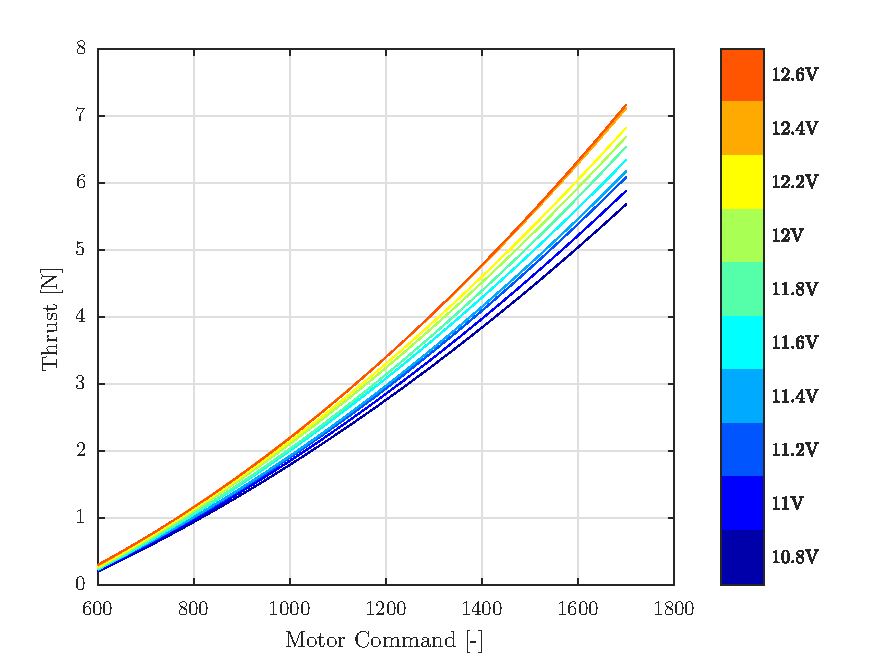
\includegraphics[width=0.8\textwidth]{img/voltage_dep_thrust_mapping.pdf}
   \caption{Second order polynomial thrust mapping (c.f.~\eqref{eq:thrust_mapping}) for different voltages between \SI{10.8}{\volt} and \SI{12.6}{\volt} identified on an ATI Mini40 load cell.}
   \label{fig:volt_dep_thrust_mapping}
\end{figure}

\begin{figure}[]
   \centering
   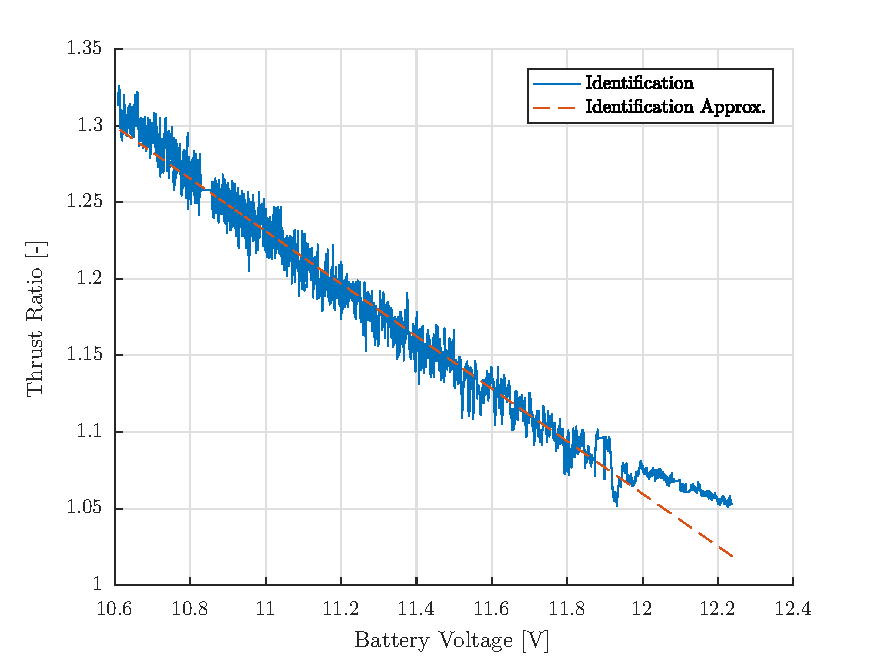
\includegraphics[width=0.8\textwidth]{img/vbat_dep_function_id.pdf}
   \caption{Estimation of thrust correction coefficient.}
   \label{fig:thrust_corr_coeff_est}
\end{figure}

\begin{figure}[]
   \centering
   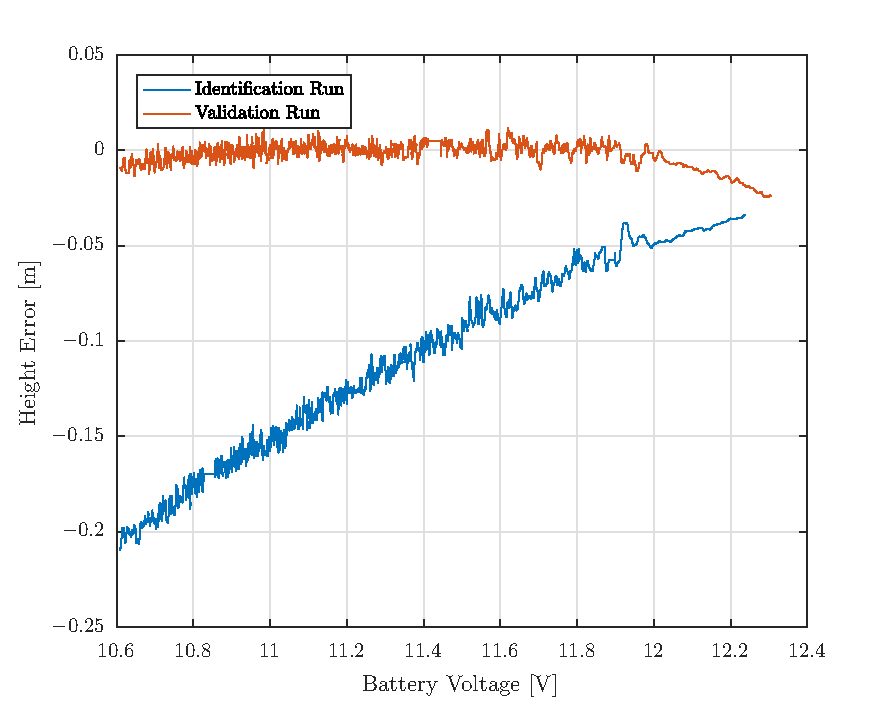
\includegraphics[width=0.8\textwidth]{img/vbat_dep_validation.pdf}
   \caption{Validation of voltage compensation.}
   \label{fig:voltage_comp_validation}
\end{figure}

\section{Trajectory Generation}

\subsection{Computing Relevant Maxima from a Reference State}

When designing a trajectory, it is often desired to enforce some limits which need to be computed from a desired state.
This section shows how to compute to most relevant values for quadrotors, namely the speed, the collective thrust, and the norm of the roll and pitch rates (especially relevant for vision-based quadrotors) as it is implemented in our \href{https://github.com/uzh-rpg/rpg_quadrotor_control/tree/master/trajectory_planning/polynomial_trajectories}{polynomial\_trajectories} library.
We assume that from a sample point on a given trajectory, we can get the reference state $\bVec{s}_{des}$ containing the position, velocity, acceleration, and jerk.
%
\begin{equation}
	\bVec{s}_{des} = \begin{bmatrix} \ori{des} & \bVec{v}_{des} & \bVec{a}_{des} & \bVec{j}_{des} \end{bmatrix}
\end{equation}

\paragraph{Speed and Collective Thrust\newline\newline}
The speed can simply be obtained by taking the norm of the reference velocity
%
\begin{equation}
	v = \norm{\bVec{v}_{des}},
\end{equation}
%
and the collective thrust can be computed as
%
\begin{equation}
	c = \norm{\bVec{a}_{des} - \bVec{g}},
\end{equation}
%
with $\bVec{g} = [0 \; 0 \; -g]^{\top}$.

\paragraph{Roll and Pitch Rate Norm\newline\newline}

We introduce the desired acceleration vector in world coordinates as
%
\begin{equation}
	\bVec{f} = \bVec{a}_{des} - \bVec{g} = \ori{WB} \cdot \begin{bmatrix}
		0 \\ 0 \\ c
	\end{bmatrix} = \ori{WB} \cdot \bVec{c},
\end{equation}
%
where $\bVec{g}$ is defined as above.
Note that $\norm{\bVec{f}} = c$ since the rotation of a vector does not change is length.
Therefore we can say
%
\begin{equation}
	\ori{WB} \cdot \begin{bmatrix}
		0 \\ 0 \\ 1
	\end{bmatrix} = \frac{\bVec{f}}{\norm{\bVec{f}}} = \bar{\bVec{f}}.
\end{equation}
%
Taking the derivative leads to
%
\begin{align}
	\ori{WB} \cdot \hat{\bodyrates} \cdot \begin{bmatrix}
		0 \\ 0 \\ 1
	\end{bmatrix} &= \dot{\bar{\bVec{f}}}, \\
	\hat{\bodyrates} \cdot \begin{bmatrix}
		0 \\ 0 \\ 1
	\end{bmatrix} &= \ori{WB}^{\top} \cdot \dot{\bar{\bVec{f}}}, \\
	\begin{bmatrix}
		\omega_y \\ -\omega_x \\ 0
	\end{bmatrix} &= \ori{WB}^{\top} \cdot \dot{\bar{\bVec{f}}},
\end{align}
%
where $\dot{\bar{\bVec{f}}}$ is computed as
%
\begin{align}
	\dot{\bar{\bVec{f}}} &= \frac{d}{dt} \left( \frac{\bVec{f}}{\norm{\bVec{f}}} \right), \\
	&= \frac{\dot{\bVec{f}} \cdot \norm{\bVec{f}} - \bVec{f} \cdot \frac{\bVec{f}^{\top} \cdot \dot{\bVec{f}}}{\norm{\bVec{f}}}}{\norm{\bVec{f}}^2}, \\
	&= \frac{\dot{\bVec{f}}}{\norm{\bVec{f}}} - \frac{\bVec{f} \cdot \bVec{f}^{\top} \cdot \dot{\bVec{f}}}{\norm{\bVec{f}}^3}, \\ 
	&= \frac{\bVec{j}}{\norm{\bVec{f}}} - \frac{\bVec{f} \cdot \bVec{f}^{\top} \cdot \bVec{j}}{\norm{\bVec{f}}^3},
\end{align}
%
using the fact that $\dot{\bVec{f}} = \bVec{j}$.
With all this we can write
\begin{align}
	\begin{bmatrix}
		\omega_y \\ -\omega_x \\ 0
	\end{bmatrix} &= \ori{WB}^{\top} \cdot \left( \frac{\bVec{j}}{\norm{\bVec{f}}} - \frac{\bVec{f} \cdot \bVec{f}^{\top} \cdot \bVec{j}}{\norm{\bVec{f}}^3} \right), \\
	&= \ori{WB}^{\top} \cdot \frac{\bVec{j}}{c} - \ori{WB}^{\top} \frac{\ori{WB} \cdot \bVec{c} \cdot \bVec{c}^{\top} \cdot \ori{WB}^{\top} \cdot \bVec{j}}{c^3}, \\
	&= \ori{WB}^{\top} \cdot \frac{\bVec{j}}{c} - \frac{\bVec{c} \cdot \bVec{c}^{\top} \cdot \ori{WB}^{\top} \cdot \bVec{j}}{c^3}.
\end{align}
%
Noting that
\begin{equation}
	\bVec{c} \cdot \bVec{c}^{\top} = \begin{bmatrix}
		0 & 0 & 0 \\
		0 & 0 & 0 \\
		0 & 0 & c^2
	\end{bmatrix},
\end{equation}
%
and using~\eqref{eq:r_basis_vectors}, we get
%
\begin{equation}
	\begin{bmatrix}
		\omega_y \\ -\omega_x \\ 0
	\end{bmatrix} = \begin{bmatrix}
		(\bVec{e}_x^B)^{\top} \cdot \frac{\bVec{j}}{c} \\
		(\bVec{e}_y^B)^{\top} \cdot \frac{\bVec{j}}{c} \\
		(\bVec{e}_z^B)^{\top} \cdot \frac{\bVec{j}}{c}
	\end{bmatrix} -
	\begin{bmatrix}
		0 \\
		0 \\
		(\bVec{e}_z^B)^{\top} \cdot \frac{\bVec{j}}{c}
	\end{bmatrix}.
\end{equation}
% 
Note that $\norm{\ori{WB}^{\top} \cdot \frac{\bVec{j}}{c}} = \norm{\frac{\bVec{j}}{c}}$ and that $\bVec{e}_z^B$ can be retrieved from the desired acceleration as
%
\begin{equation}
	\bVec{e}_z^B = \frac{\bVec{a}_{des} - \bVec{g}}{\norm{\bVec{a}_{des} - \bVec{g}}}.
\end{equation}
%
Therefore, we can compute the norm of the roll and pitch body rates as
%
\begin{equation}
	\norm{\omega_{x,y}} = \norm{\begin{bmatrix}
		\omega_y \\ -\omega_x \\ 0
	\end{bmatrix}} = \sqrt{\norm{\frac{\bVec{j}}{c}}^2 - \left( (\bVec{e}_z^B)^{\top} \cdot \frac{\bVec{j}}{c} \right)^2}
\end{equation}

\section{Math}

\subsection{Mechanics}

\subsubsection{Euler's first law}

The linear momentum of a rigid body, $\bVec{p}$ is defined as 
%
\begin{equation}
	 \bVec{p} := m\cdot   \bVec{v}_S,
	 \label{eq:linear_momentum}
\end{equation}
%
where $m$ is the mass of the body, and $\bVec{v}_S$ is the velocity of the center of mass.
Euler's first law states that the change of linear momentum is equal to the sum of all external forces $\bVec{F}$:
%
\begin{equation}
	\dot{\bVec{p}} =   \bVec{F},
	\label{eq:sum_of_all_forces_equal_dp}
\end{equation}
%
Differentiating~\eqref{eq:linear_momentum} and inserting in~\eqref{eq:sum_of_all_forces_equal_dp} gives
%
\begin{equation}
	\dot{\bVec{p}} = m \cdot   \bVec{a}_S =   \bVec{F},
	\label{eq:pdot_equal_F}
\end{equation}
%
where $\bVec{a}_S$ is the acceleration of the center of mass.	

\subsubsection{Euler's second law}	

The angular momentum of a rigid body with respect to a stationary point $O$ is defined as 
%
\begin{equation}
	\vect{L}{}{O} :=   \ori{OP} \times   \bVec{p} + \vect{I}{}{P} \cdot   \bVec{\Omega} + m \cdot   \ori{PS}\times \vect{v}{}{P},
	\label{eq:L_O_P}
\end{equation}
%
where $P$ is an arbitrary point on the body, and $\vect{I}{}{P}$ is the second moment of inertia matrix with respect to a rotation around $P$, $\bVec{\Omega} $ is the angular velocity of the body.
Evaluating~\eqref{eq:L_O_P} not for an arbitrary $P$ but at the center of mass $P=S$ we find
%
\begin{equation}
	\vect{L}{}{O} =   \ori{OS} \times    \bVec{p} +  \vect{I}{}{S} \cdot  \bVec{\Omega}.
	\label{eq:L_O_S}
\end{equation}
%
Euler's second law states that the change of angular momentum is equal to the sum of all external moments $\vect{M}{}{O}$ with respect to $O$:
% 
\begin{equation}
	\vectdot{L}{}{O} = \vect{M}{}{O}.
	\label{eq:second_law}
\end{equation}
%
Differentiating~\eqref{eq:L_O_S} and inserting in~\eqref{eq:second_law} gives
%
\begin{equation}
	\vectdot{L}{}{O} = \ori{OS}\times  \dot{\bVec{p}} + \vect{I}{}{S} \cdot   \bVec{\Psi} + \bVec\Omega \times   \vect{I}{}{S} \cdot   \bVec{\Omega}  =   \vect{M}{}{O},
	\label{ldot_equal_MO}
\end{equation}
%
where $\bVec{\Psi}$ is the angular acceleration of the body.
We can further rewrite~\eqref{ldot_equal_MO} as
%
\begin{align}
  \vectdot{L}{}{O} -   \ori{OS}\times  \dot{\bVec{p}} = 
  \vect{I}{}{S} \cdot   \bVec{\Psi} + 
  \bVec\Omega \times   \vect{I}{}{S} \cdot   \bVec{\Omega} & = 
  \vect{M}{}{O}-   \ori{OS}\times  \dot{\bVec{p}}, \nonumber\\
%%%%%%%%%%%%%%%%%%%%%%%%%%%%%%%%%%%%%%%%%%%%%%%%
%=  \vect{I}{}{S} \cdot   \bVec{\Psi} +
%  \bVec\Omega \times   \vect{I}{}{S} \cdot   \bVec{\Omega}
& = 
  \vect{M}{}{O} +   \ori{SO}\times  \dot{\bVec{p}}, \nonumber\\
%%%%%%%%%%%%%%%%%%%%%%%%%%%%%%%%%%%%%%%%%%%%%%%%
%=   \vect{I}{}{S} \cdot   \bVec{\Psi} +
%  \bVec\Omega \times   \vect{I}{}{S} \cdot   \bVec{\Omega}
& = 
  \vect{M}{}{O} +   \ori{SO}\times  \bVec{F}, \nonumber\\
%%%%%%%%%%%%%%%%%%%%%%%%%%%%%%%%%%%%%%%%%%%%%%%%
  \vect{I}{}{S} \cdot   \bVec{\Psi} + 
  \bVec\Omega \times   \vect{I}{}{S} \cdot   \bVec{\Omega} & = 
  \vect{M}{}{S}.
	\label{eq:ldot_equal_MS}
\end{align}

\subsubsection{Differentiating the Angular Momentum}

This section shows how to differentiate $ \vect{L}{}{O} $.
First, we restate~\eqref{eq:L_O_S} for the definition of the angular momentum
%
\begin{equation}
	\vect{L}{}{O} = \ori{OS} \times \bVec{p} + \vect{I}{}{S} \cdot \bVec{\Omega} .
	\label{eq:L_O_S_2}
\end{equation}
%
Later we will use Euler's differentiation rule, therefore we restate it here. 
Euler's differentiation rule is used to differentiate in a body fixed coordinate system $\bfr$
%
\begin{equation}
	\vectdot{c}{\bfr}{} =
	\left( \vect{\thrust}{\bfr}{} \right)' + \vect{\bodyrates}{\wfr}{\wfr \bfr}  \times \vect{\thrust}{\bfr}{} .
	\label{eq:app_euler_rule}
\end{equation}
%
Note the special notation for $ \left( \vect{\thrust}{\bfr}{} \right)' $ which is just the  differentiation over time of $ \vect{\thrust}{\bfr}{} $ which is different than the differentiation expressed in the $\bfr$ system $ \vectdot{c}{\bfr}{} $.
Now, lets start to calculate $\vectdot{L}{}{O}$. 
For better readability we differentiate the two terms in~\eqref{eq:L_O_S_2} separately:
%
\begin{align}
	\dot{ \left( \ori{OS} \times \bVec{p} \right) } & = 
	\vectdot{\ori{}}{}{OS} \times \bVec{p} + 
	\ori{OS} \times \dot{ \bVec{p} }, \\
	& = 
	v_{S} \times \bVec{p} +
	\ori{OS} \times \dot{ \bVec{p} }, \\
	& = 
	v_{S} \times m \cdot v_{S} + 
	\ori{OS} \times \dot{ \bVec{p} }, \\
	& = 
	\ori{OS} \times \dot{ \bVec{p} }.
	\label{eq:appendix_drall_deriv0}
\end{align}
%
To differentiate $ \vect{I}{}{S} \cdot \bVec{\Omega} $ we evaluate it in the body fixed coordinate system $\bfr$. 
We do this because the second moment of inertia matrix $\vect{I}{B}{S}$ is constant in a body fixed frame
%
\begin{align}
	\prescript{}{\bfr}{\dot{ \left( \vect{I}{}{S} \cdot \bVec{\Omega} \right)} } 
	& =
	\left( \vect{I}{B}{S} \vect{\Omega}{\bfr}{} \right)'
	+ \vect{\Omega}{\bfr}{} \times \vect{I}{B}{S} \cdot \vect{\Omega}{\bfr}{}, \\
	& = 
	\cancelto{0}{\left( \vect{I}{B}{S}  \right)'} \vect{\Omega}{\bfr}{} +
	 \vect{I}{B}{S}  \left( \vect{\Omega}{\bfr}{} \right)'
	+ \vect{\Omega}{\bfr}{} \times \vect{I}{B}{S} \cdot \vect{\Omega}{\bfr}{}, \\
	& = 
	\vect{I}{B}{S}  \left( \vect{\Omega}{\bfr}{} \right)'
	+ \vect{\Omega}{\bfr}{} \times \vect{I}{B}{S} \cdot \vect{\Omega}{\bfr}{}.
	\label{eq:appendix_drall_deriv1}
\end{align}
%
To rewrite $ \left( \vect{\Omega}{\bfr}{} \right)' $ we differentiate the angular velocity of the body using euler's formula~\eqref{eq:app_euler_rule}
%
\begin{align}
	\vectdot{\Omega}{\bfr}{}
	&=
	\left( \vect{\Omega}{\bfr}{} \right)' + 
	\vect{\bodyrates}{\wfr}{\wfr \bfr}  \times \vect{\Omega}{\bfr}{}, \\
	&= 	
	\left( \vect{\Omega}{\bfr}{} \right)' + 
	\cancelto{0}{ \vect{\Omega}{\bfr}{}  \times \vect{\Omega}{\bfr}{} }, \\
	&=
	\left( \vect{\Omega}{\bfr}{} \right)'. \label{eq:app_body_rates_dev}
\end{align}
%
Inserting~\eqref{eq:app_body_rates_dev} in~\eqref{eq:appendix_drall_deriv1} we can continue with the differentiation of the second term
%
\begin{align}
	\prescript{}{\bfr}{\dot{ \left( \vect{I}{}{S} \cdot \bVec{\Omega} \right) }}
	& =
	\vect{I}{B}{S} \vectdot{\Omega}{\bfr}{} 
	+ \vect{\Omega}{\bfr}{} \times \vect{I}{B}{S} \cdot \vect{\Omega}{\bfr}{}.
	\label{eq:appendix_drall_deriv2}
\end{align}
%
This result is valid in any coordinate system not only the body fixed, therefore we can write~\eqref{eq:appendix_drall_deriv2} as
%
\begin{align}
	\dot{ \left( \vect{I}{}{S} \cdot \bVec{\Omega} \right) } 
	& =
	\vect{I}{}{S} \dot{\bVec{\Omega}} 
	+ \bVec{\Omega} \times \vect{I}{}{S} \cdot \bVec{\Omega}.
	\label{eq:appendix_drall_deriv3}
\end{align}
%
Combining the results~\eqref{eq:appendix_drall_deriv0} and~\eqref{eq:appendix_drall_deriv3} we finally find
%
\begin{align}
	\dot{ \bVec{L}} _O
	& = 
	\ori{OS} \times \dot{ \bVec{p} } + 
	\vect{I}{}{S} \dot{\bVec{\Omega}} 
	+ \bVec{\Omega} \times \vect{I}{}{S} \cdot \bVec{\Omega}, \\	
	& = 
	\ori{OS} \times \dot{ \bVec{p} } + 
	\vect{I}{}{S} \bVec{\Psi} 
	+ \bVec{\Omega} \times \vect{I}{}{S} \cdot \bVec{\Omega}.
\end{align}
%
Again this result is valid in any coordinate system.

\subsubsection{Summary}

Note that we can not only evaluate~\eqref{eq:pdot_equal_F} and~\eqref{eq:ldot_equal_MS} in the world frame $\wfr$ but in any rotating coordinate systems $A$ and $C$.
%
\begin{align}
	m \cdot \vect{a}{A}{S} & = \vect{F}{A}{}, \\
	\vect{I}{C}{S} \cdot  \prescript{}{C}{\bVec{\Psi}} + \vect{\Omega}{C}{} \times  \vect{I}{C}{S} \cdot \vect{\Omega}{C}{} &= \vect{M}{C}{S}.
\end{align}

\subsection{Attitude Representations}

This is not an introduction to coordinate transformations but a small summary of the important math we need to describe the dynamics of a quadrotor.

\subsubsection{Rotation Matrices and Euler Angles}\label{sec:traforotmat}

We denote the rotation matrix that converts from system $\bfr$ to $\wfr$ as $\ori{\wfr \bfr}$ and the translation of system $\bfr$ with respect to system $\wfr$ as $\bVec{t}_{\wfr \bfr}$, respectively.
To convert a vector $\bVec{c}$ from the body frame $\bfr$ to the world frame $\wfr$ we use
%
\begin{equation}
	\vect{\thrust}{\wfr}{} = \ori{\wfr \bfr} \cdot \vect{\thrust}{\bfr}{} .
\end{equation}
%
Correspondingly, to convert a point $\bVec{p}$ from the body frame $\bfr$ to the world frame $\wfr$ we use
%
\begin{equation}
	\vect{\pos}{\wfr}{} = \ori{\wfr \bfr} \cdot \vect{\pos}{\bfr}{} \; + \; \vect{t}{\wfr}{\wfr \bfr} .
\end{equation}
%
Later on Euler angles can be used.
It is really important to keep in mind that with Euler angles the order of each single rotation is important. 
When you are using formulas with euler angles, always check what convention they are using.
Here we will use the $z-y-x$ convention:
%
\begin{enumerate}
\item yaw $\psi$ around the z body axis
\item pitch $\theta$ around the new y body axis
\item roll $\phi$ around the new x body axis
\end{enumerate}
%
\begin{equation}
	\ori{\wfr \bfr} = \ori{z}(\psi) \ori{y}(\theta) \ori{x}(\phi) ,	
\end{equation}
%
where
% 
\begin{align}
\ori{z}(\psi) &= 
\begin{bmatrix} 
	\cos (\psi) & -\sin (\psi) & 0 \\
	\sin (\psi) & \cos (\psi) & 0 \\
	0 & 0 & 1 \\	
\end{bmatrix},
\\
\ori{y}(\theta) &= 
\begin{bmatrix} 
	\cos (\theta) & 0 & \sin (\theta) \\
	0 & 1 & 0 \\
	-\sin (\theta) & 0 & \cos (\theta)
\end{bmatrix},
\\
\ori{x}(\phi) &= 
\begin{bmatrix} 
	1 & 0 & 0 \\
	0 & \cos (\phi) & -\sin (\phi) \\
	0 & \sin (\phi) & \cos (\phi) \\
\end{bmatrix}.
\end{align}
%
Putting it all together we get
%
\begin{align}
\ori{\wfr \bfr} &= \begin{bmatrix}
\scos(\psi)\scos(\theta) & \scos(\psi)\ssin(\theta)\ssin(\phi)-\ssin(\psi)\scos(\phi) & \scos(\psi)\ssin(\theta)\scos(\phi)+\ssin(\psi)\ssin(\phi) \\
\ssin(\psi)\scos(\theta) & \ssin(\psi)\ssin(\theta)\ssin(\phi)+\scos(\psi)\scos(\phi) & \ssin(\psi)\ssin(\theta)\scos(\phi)-\scos(\psi)\ssin(\phi) \\
-\ssin(\theta) & \scos(\theta)\ssin(\phi) & \scos(\theta)\scos(\phi)
\end{bmatrix}, \\
	&= \begin{bmatrix} \vect{x}{}{\bfr} & \vect{y}{}{\bfr} & \vect{z}{}{\bfr} \end{bmatrix}, \label{eq:r_basis_vectors}
\end{align}
%
with $\vect{x}{}{\bfr}$, $\vect{y}{}{\bfr}$ and $\vect{z}{}{\bfr}$ being the orthogonal basis vectors of the Body coordinate system $\bfr$ represented in world coordinates $\wfr$ as illustrated in Fig.~\ref{fig:quad}.
The angular velocity of coordinate system $\bfr$ with respect to the world frame $\wfr$ is denoted as $\vect{\bodyrates}{}{\wfr \bfr}$. 
For the next step, we define the skew symmetric matrix
%
\begin{equation}
\vect{\hat{\bodyrates}}{}{\wfr \bfr} = 
	\begin{bmatrix} 
    	0 & -\omega_{3} & \omega_{2}\\
    	\omega_{3}& 0 &-\omega_{1}\\
    	-\omega_{2} & \omega_{1} & 0 
    \end{bmatrix} .
\end{equation}
%
The angular velocity is defined as
%
\begin{equation}
\vect{\hat{\bodyrates}}{\wfr}{\wfr \bfr} := \vectdot{\ori{}}{}{\wfr \bfr} \cdot \ori{\wfr \bfr}^{T} ,
\label{eq:I_omegahat_IB}
\end{equation}
%
or in body frame $\bfr$
%
\begin{align}
\vect{\hat{\bodyrates}}{\bfr}{\wfr \bfr} 
&= 
\ori{\bfr\wfr} \cdot \vect{\hat{\bodyrates}}{\wfr}{\wfr \bfr} \cdot \ori{\bfr \wfr}^{T}, \\
& = \ori{\bfr \wfr} \cdot \vectdot{\ori{}}{}{\wfr \bfr} \cdot \ori{\wfr \bfr}^{T}  \cdot \ori{\bfr \wfr}^{T}, \\
& = \ori{\wfr \bfr}^{\top} \cdot \vectdot{\ori{}}{}{\wfr \bfr}.
\label{eq:B_omegahat_IB}
\end{align}
%
Evaluating~\eqref{eq:I_omegahat_IB} and~\eqref{eq:B_omegahat_IB} for $\vect{\bodyrates}{}{\wfr \bfr}$ we get
%        
\begin{equation}
\vect{\bodyrates}{\wfr}{\wfr \bfr} =
\begin{bmatrix} \dot{\phi} \scos(\theta) \scos(\psi) - \dot{\theta} \ssin(\psi) \\
\dot{\phi} \scos(\theta) \ssin(\psi) + \dot{\theta} \scos(\psi) \\
-\dot{\phi} \ssin(\theta) + \dot{\psi} 
\end{bmatrix} 
= 
\begin{bmatrix} \scos(\theta) \scos(\psi) & -\ssin(\psi) & 0 \\
\scos(\theta) \ssin(\psi) & \scos(\psi) & 0 \\
-\ssin(\theta) & 0 & 1
\end{bmatrix} 
\begin{bmatrix}
	\dot{\phi}\\
	\dot{\theta}\\
	\dot{\psi}
\end{bmatrix} ,
\label{eq:I_omega_IB}
\end{equation}
%
and
%
\begin{equation}
\vect{\bodyrates}{\bfr}{\wfr \bfr} =
\begin{bmatrix}
	\dot{\phi} - \ssin(\theta) \dot{\psi} \\
	\scos(\phi) \dot{\theta} + \ssin(\phi)\scos(\theta) \dot{\psi}\\
	-\ssin(\phi) \dot{\theta} + \scos(\phi)\scos(\theta) \dot{\psi}
\end{bmatrix}
=
\begin{bmatrix}
	1 & 0 & -\ssin(\theta) \\
	0 & \scos(\phi) & \ssin(\phi)\scos(\theta) \\
	0 & -\ssin(\phi) & \scos(\phi)\scos(\theta)
\end{bmatrix}
\begin{bmatrix}
	\dot{\phi}\\
	\dot{\theta}\\
	\dot{\psi}
\end{bmatrix} .
\label{eq:B_omega_IB}
\end{equation}

\subsubsection{Quaternions}\label{sec:trafoquaternion}

Instead of using Euler angles or rotation matrices, the orientation of a quadrotor can also be represented as a quaternion. 
We denote
%
\begin{equation}
\vect{q}{}{\wfr \bfr} = \begin{bmatrix} \qw & \qx & \qy & \qz \end{bmatrix}^{\top} \label{eq:quat_convention}
\end{equation}
%
as the quaternion that describes the orientation of coordinate frame $\bfr$ with respect to coordinate frame $\wfr$, where $q_w$ is the real part of the quaternion. 
Note that $\vect{q}{}{\wfr \bfr}$ is what you get from optitrack. 
The adjoint, norm, and inverse of the quaternion, $\bVec{q}$, are 
% 
\begin{align}
	\bar{\bVec{q}} &= \begin{bmatrix} \qw & -\qx & -\qy & -\qz \end{bmatrix}^{\top},\\
	 \norm{\bVec{q}} & =  \sqrt{ \qw^2 + \qx^2 + \qy^2 + \qz^2 },\\
	 \bVec{q}^{-1} & = \frac{ \bar{\bVec{q}} }{ \norm{\bVec{q}}  }.
\end{align}
%
\paragraph{Quaternion Multiplication}

Quaternion multiplication is not commutative. 
The Quaternion multiplication between quaternions $\bVec{q}$ and $\bVec{p}$ is defined as
%
\begin{align}
\bVec{q} \otimes \bVec{p} = \bVec{Q}\left(\bVec{q}\right) \cdot \bVec{p} = \bar{\bVec{Q}}\left(\bVec{p}\right) \cdot \bVec{q},\\
%
\bVec{p} \otimes \bVec{q} = \bVec{Q}\left(\bVec{p}\right) \cdot \bVec{q} = \bar{\bVec{Q}}\left(\bVec{q}\right)\cdot \bVec{p},\\
\end{align}
%
where 
%
\begin{equation}
\bVec{Q}\left(\bVec{q}\right) = 
\begin{bmatrix} 
	\qw & -\qx & -\qy & -\qz \\ 
	\qx &  \qw & -\qz &  \qy \\
	\qy &  \qz &  \qw & -\qx \\
	\qz & -\qy &  \qx &  \qw \\
\end{bmatrix},
\end{equation}
%
\begin{equation}
\bar{\bVec{Q}}\left(\bVec{q}\right) = 
\begin{bmatrix} 
	\qw & -\qx & -\qy & -\qz \\ 
	\qx &  \qw &  \qz & -\qy \\
	\qy & -\qz &  \qw &  \qx \\
	\qz &  \qy & -\qx &  \qw \\
\end{bmatrix}.
\end{equation}
%
We find that
%
\begin{align}
\bVec{Q}\left(\bar{\bVec{q}}\right) = \bVec{Q}\left(\bVec{q}\right)^{\top},\\
\bar{\bVec{Q}}\left(\bar{\bVec{q}}\right) = \bar{\bVec{Q}}\left(\bVec{q}\right)^{\top}.
\end{align}

\paragraph{Rotating a Vector by a Quaternion}

To rotate a vector $\bVec{v}$ by a quaternion $\bVec{q}$ we use the notion $\bVec{q} \odot \bVec{v}$. 
To rotate a vector $\prescript{}{\bfr}{\bVec{v}}$ represented in body coordinates $\bfr$ into world coordinates $\wfr$ we can apply
%
\begin{equation}
	\begin{bmatrix} 0 \\ \vect{\vel}{\wfr}{} \end{bmatrix} = \begin{bmatrix} 0 \\ \vect{q}{}{\wfr \bfr} \odot \vect{\vel}{\bfr}{} \end{bmatrix} = \bar{\bVec{Q}}^{\top} \left(\vect{q}{}{\wfr \bfr}\right) \cdot \bVec{Q}\left(\vect{q}{}{\wfr \bfr}\right) \cdot \begin{bmatrix} 0 \\ \vect{\vel}{\bfr}{} \end{bmatrix} .
\end{equation}
%
This equation will be more clear by looking at the derivations for transforming a quaternion into a rotation matrix as described in Section~\ref{sec:quat_to_tor_mat}.

\paragraph{Quaternion Rates to Angular Velocity}

The time derivative of the unit quaternion is the vector of quaternion rates. 
The quaternion rates $\dot{\bVec{q}}$ are related to the angular velocities similar to~\eqref{eq:I_omegahat_IB}.
%
\begin{align}
\begin{bmatrix}
	0\\
	\vect{\bodyrates}{\wfr}{\wfr \bfr}
\end{bmatrix}
&=
2 \vectdot{q}{}{\wfr \bfr} \otimes \vectbar{q}{}{\wfr \bfr},
\\&= 
2 \bVec{Q}\left( \vectdot{q}{}{\wfr \bfr} \right) \vectbar{q}{}{\wfr \bfr},
\\&=
2 \bar{\bVec{Q}}\left( \vectbar{q}{}{\wfr \bfr} \right) \vectdot{q}{}{\wfr \bfr},
\end{align}
%
or in body fixed frame $\bfr$
%
\begin{align}
\begin{bmatrix}
	0\\
	\vect{\bodyrates}{\wfr}{\wfr \bfr}
\end{bmatrix}
&=
2 \vectbar{q}{}{\wfr \bfr} \otimes \vectdot{q}{}{\wfr \bfr}.
\label{eq:omega_from_q_body}
\end{align}
%
More compactly, we can write
%
\begin{align}
\vect{\bodyrates}{\wfr}{\wfr \bfr} = 2\bVec{W}\left( \vect{q}{}{\wfr \bfr} \right) \vectdot{q}{}{\wfr \bfr},\\
\vect{\bodyrates}{\wfr}{\wfr \bfr} = 2\bVec{W'}\left( \vect{q}{}{\wfr \bfr} \right) \vectdot{q}{}{\wfr \bfr},
\end{align}
%
with $\bVec{W} \left( \vect{q}{}{\wfr \bfr} \right)$ and $\bVec{W'}\left( \vect{q}{}{\wfr \bfr} \right)$ as defined in Section~\ref{sec:quat_to_tor_mat}.

\subsubsection{Changing Transformation Representation}

This section lists the common conversions between different orientation representations.

\paragraph{Rotation Matrix to Euler Angles}

For this conversion, we denote $R_{ij}$ as the element in row $i$ and column $j$ of $\ori{\wfr \bfr}$.
%
\begin{align}
	\phi &= \atantwo(R_{32}, R_{33}) \\
	\theta &= \atantwo(R_{31}, \sqrt{R_{32}^2 + R_{33}^2}) \\
	\psi &= \atantwo(R_{21}, R_{11})
\end{align}

\paragraph{Euler Angles to Rotation Matrix}

\begin{equation}
\ori{\wfr \bfr} = \begin{bmatrix}
\scos(\psi)\scos(\theta) & \scos(\psi)\ssin(\theta)\ssin(\phi)-\ssin(\psi)\scos(\phi) & \scos(\psi)\ssin(\theta)\scos(\phi)+\ssin(\psi)\ssin(\phi) \\
\ssin(\psi)\scos(\theta) & \ssin(\psi)\ssin(\theta)\ssin(\phi)+\scos(\psi)\scos(\phi) & \ssin(\psi)\ssin(\theta)\scos(\phi)-\scos(\psi)\ssin(\phi) \\
-\ssin(\theta) & \scos(\theta)\ssin(\phi) & \scos(\theta)\scos(\phi)
\end{bmatrix}
\end{equation}

\paragraph{Quaternion to Euler Angles}

\begin{align}
	\phi &= \atantwo(2 q_w q_x + 2 q_y q_z, \; q_w^2 - q_x^2 - q_y^2 + q_z^2) \\
	\theta &= -\asin(2 q_x q_z - 2 q_w q_y) \\
	\psi &= \atantwo(2 q_w q_z + 2 q_x q_y, \; q_w^2 + q_x^2 - q_y^2 - q_z^2)
\end{align}

\paragraph{Euler Angles to Quaternion}

\begin{equation}
	\vect{q}{}{\wfr \bfr} = \begin{bmatrix} q_w \\ q_x \\ q_y \\ q_z	\end{bmatrix} 
	= \begin{bmatrix} \cos\left(\frac{\phi}{2}\right) \cos\left(\frac{\theta}{2}\right) \cos\left(\frac{\psi}{2}\right) + \sin\left(\frac{\phi}{2}\right) \sin\left(\frac{\theta}{2}\right) \sin\left(\frac{\psi}{2}\right) \\
	\sin\left(\frac{\phi}{2}\right) \cos\left(\frac{\theta}{2}\right) \cos\left(\frac{\psi}{2}\right) - \cos\left(\frac{\phi}{2}\right) \sin\left(\frac{\theta}{2}\right) \sin\left(\frac{\psi}{2}\right) \\
	\cos\left(\frac{\phi}{2}\right) \sin\left(\frac{\theta}{2}\right) \cos\left(\frac{\psi}{2}\right) + \sin\left(\frac{\phi}{2}\right) \cos\left(\frac{\theta}{2}\right) \sin\left(\frac{\psi}{2}\right) \\
	\cos\left(\frac{\phi}{2}\right) \cos\left(\frac{\theta}{2}\right) \sin\left(\frac{\psi}{2}\right) - \sin\left(\frac{\phi}{2}\right) \sin\left(\frac{\theta}{2}\right) \cos\left(\frac{\psi}{2}\right) \\
	 \end{bmatrix}
\end{equation}

\paragraph{Quaternion to Rotation Matrix} \label{sec:quat_to_tor_mat}

Unit quaternions are quaternions with unity norm. 
Throughout this section, we assume that
%
\begin{equation}
	\| \bVec{q} \| = 1 .
\end{equation}
%
To convert a vector $\bVec{c}$ from the body frame $\bfr$ to the world frame $\wfr$ we use
%
\begin{align}
\begin{bmatrix} 
	0\\
	\vect{\thrust}{\wfr}{}
\end{bmatrix}
& = 
\bVec{q} \cdot
\begin{bmatrix} 
	0\\
	\vect{\thrust}{\bfr}{}
\end{bmatrix} \cdot
\bVec{q}^{-1},\\
%
& = 
\bVec{q} \cdot
\begin{bmatrix} 
	0\\
	\vect{\thrust}{\bfr}{}
\end{bmatrix} \cdot
\bar{\bVec{q}},\\
% 
&= 
\bar{\bVec{Q}}\left(\bVec{q}\right)^{\top}
\bVec{Q}\left(\bVec{q}\right)
\begin{bmatrix} 
	0\\
	\vect{\thrust}{\bfr}{}
\end{bmatrix}, \label{eq:d123}\\
%
&=
\begin{bmatrix} 
	1        & \bVec{0}^{\top}\\
    \bVec{0} & \ori{\wfr \bfr}
\end{bmatrix} 
\begin{bmatrix} 
	0\\
	\vect{\thrust}{\bfr}{} 
\end{bmatrix}. \label{eq:d124}
\end{align}
%
From~\eqref{eq:d123} and~\eqref{eq:d124}, it can be seen that the rotation matrix can be as
%
\begin{equation}
\ori{\wfr \bfr}
=
\begin{bmatrix} 
\qw^2 + \qx^2 - \qy^2 - \qz^2, & 2\qx\qy - 2\qw\qz,         & 2\qw\qy + 2\qx\qz\\
2\qw\qz + 2\qx\qy,         & \qw^2 - \qx^2 + \qy^2 - \qz^2, & 2\qy\qz - 2\qw\qx\\
2\qx\qz - 2\qw\qy,         & 2\qw\qx + 2\qy\qz,         & \qw^2 - \qx^2 - \qy^2 + \qz^2\\
\end{bmatrix}.
\label{eq:quatToRot}
\end{equation}
%
To rewrite~\eqref{eq:d123} and~\eqref{eq:d124}, we define
%
\begin{equation}
	\bVec{W}(\vect{q}{}{\wfr \bfr}) = \begin{bmatrix} 
	-q_x & q_w & -q_z & q_y \\
	-q_y & q_z & q_w & -q_x \\
	-q_z & -q_y & q_x & q_w 
	\end{bmatrix},
\end{equation}
%
\begin{equation}
	\bVec{W'}(\vect{q}{}{\wfr \bfr}) = \begin{bmatrix} 
	-q_x & q_w & q_z & -q_y \\
	-q_y & -q_z & q_w & q_x \\
	-q_z & q_y & -q_x & q_w 
	\end{bmatrix},
\end{equation}
%
which allows us to write~\eqref{eq:quatToRot} as
%
\begin{align}
\ori{\wfr \bfr} = \bVec{W}(\vect{q}{}{\wfr \bfr}) \bVec{W'}(\vect{q}{}{\wfr \bfr})^{\top} .
\end{align}
%
Note that just as with rotation matrices, sequences of rotations are represented by products of quaternions. 
That is, for unit quaternions it holds that
%
\begin{equation}
	\ori{}\left( \bVec{q} \cdot \bVec{p} \right) = 
	\ori{}\left( \bVec{q} \right) \ori{}\left( \bVec{p} \right).
\end{equation}
%
%Furthermore we define the following matrices.
%
%Correspondingly, to convert a point $\bVec{p}$ from the body frame $B$ to the world frame $\wfr$ we use
%
%\begin{equation}
%	{_\wfr}\bVec{p} = \bVec{W}(\bVec{q}_{\wfr B}) \cdot \bVec{W'}(\bVec{q}_{\wfr B})^{\top} \cdot {_B}\bVec{p} \; + \; {_\wfr}\bVec{t}_{\wfr B}
%	\label{eq:quattranspoint}
%\end{equation}
%
%where $\bVec{t}_{\wfr B}$ denotes the translation of coordinate frame $B$ with %respect to coordinate frame $\wfr$.
%
Getting a quaternion directly from a rotation matrix is not straight forward but is also not used very often in our applications and if, we let \href{http://eigen.tuxfamily.org/index.php?title=Main_Page}{Eigen} do it.

\subsection{Classical Modeling of a Quadrotor} \label{sec:dynamics}

\subsubsection{Using Euler Angles}\label{sec:dynamicseuler}

In this section we use Euler angles and the corresponding rotation matrices as defined in Section~\ref{sec:traforotmat}, where the rotation matrix $\ori{\wfr \bfr}(\phi, \theta, \psi)$ is a function of the euler angles.
\newline\newline
We can evaluate~\eqref{eq:pdot_equal_F} in the world frame as
%
\begin{equation}
	\sVec{\ddot{x}\\ \ddot{y} \\ \ddot{z}} =  
\sVec{0\\ 0\\ - g} + \ori{\wfr \bfr}(\phi, \theta, \psi) \sVec{0\\ 0\\ c},
	\label{eq:lindynamics}
\end{equation}
%
or in vectorized form
%
\begin{equation}
	\ddot{\pos} = \vect{\gravityvec}{\wfr}{} + \ori{\wfr \bfr}(\phi, \theta, \psi) \cdot \bVec{c}.
\end{equation}
%
Next, we evaluate~\eqref{eq:ldot_equal_MS} in the body coordinate system $\bfr$
%
\begin{align}
	\begin{bmatrix} 
    	J_{xx} & 0 & 0 \\ 0 & J_{yy} & 0 \\ 0 & 0 & J_{zz} 
    \end{bmatrix}  
    \sVec{\dot{p}\\ \dot{q} \\ \dot{r}}  
    + 
	\sVec{p \\ q\\ r} 
	\times  
	\begin{bmatrix} 
		J_{xx} & 0 & 0 \\ 0 & J_{yy} & 0 \\ 0 & 0 & J_{zz} 
	\end{bmatrix} 
	\sVec{p \\ q\\ r} 
&= 
 \begin{bmatrix} \frac{\sqrt{2}}{2}l(f_1-f_2-f_3+f_4) \\
							\frac{\sqrt{2}}{2}l(-f_1-f_2+f_3+f_4) \\
							\kappa(f_1-f_2+f_3-f_4)
						\end{bmatrix} ,
\\
\begin{bmatrix} 
       J_{xx} \dot{p} + q \cdot r \left( J_{zz} - J_{yy} \right)\\
       J_{yy} \dot{q} + p \cdot r \left( J_{xx} - J_{zz} \right)\\
       J_{zz} \dot{r} + p \cdot q \left( J_{yy} - J_{xx} \right)
\end{bmatrix}   
  &= 
 \begin{bmatrix} \frac{\sqrt{2}}{2}l(f_1-f_2-f_3+f_4) \\
							\frac{\sqrt{2}}{2}l(-f_1-f_2+f_3+f_4) \\
							\kappa(f_1-f_2+f_3-f_4)
						\end{bmatrix},
\label{eq:rotdynamics}
\end{align}
%
or in vectorized form
%
\begin{equation}
	\bVec{J} \cdot \vectdot{\bodyrates}{\bfr}{\wfr \bfr} + \vect{\bodyrates}{\wfr}{\wfr \bfr} \times \bVec{J} \cdot   \vect{\bodyrates}{\wfr}{\wfr \bfr} = \bodytorques .
	\label{eq:rotdynamicsvector}
\end{equation}
%
Now, we want to write the quadrotor dynamics in state space form. 
First, we chose the state vector as
%
\begin{align}
	\bVec{s} &= \begin{bmatrix} x & y &z &\dot{x} &\dot{y} &\dot{z} &\phi &\theta &\psi &p &q &r \end{bmatrix}^{\top} ,\label{eq:state} \\
	&= \begin{bmatrix} \vect{\pos}{\wfr}{\wfr \bfr} & \vect{\vel}{\wfr}{\wfr \bfr} & \phi & \theta & \psi & \vect{\bodyrates}{\wfr}{\wfr \bfr} \end{bmatrix}^{\top} .
\end{align}
%
In the following we rewrite~\eqref{eq:lindynamics} and~\eqref{eq:rotdynamics} in order to fit the state space form. 
%
\begin{align}
\begin{bmatrix} 
	\dot{x} \\\dot{y} \\\dot{z} 
\end{bmatrix}
	&= \begin{bmatrix} 
	\dot{x} \\\dot{y} \\\dot{z} 
\end{bmatrix}, \\
%
\begin{bmatrix} 
	\ddot{x} \\\ddot{y} \\\ddot{z} 
\end{bmatrix}
	&= \begin{bmatrix} 0\\ 0\\ -g\end{bmatrix} + \ori{\wfr \bfr}(\phi, \theta, \psi) \begin{bmatrix} 0\\ 0\\ c \end{bmatrix},	\\
%
\begin{bmatrix}
	\dot{\phi} \\ \dot{\theta} \\ \dot{\psi} 
\end{bmatrix} 
 &=
\begin{bmatrix} 1 & \stan(\theta)\ssin(\phi) & \stan(\theta)\scos(\phi) \\ 
0 & \scos(\phi) & -\ssin(\phi) 
\\ 0 & \frac{\ssin(\phi)}{\scos(\theta)}  & \frac{\scos(\phi)}{\scos(\theta)} \end{bmatrix}    
\begin{bmatrix}
	p \\ q \\ r 
\end{bmatrix}, \label{eq:euleranglerates} \\
%
\begin{bmatrix} 
	\dot{p} \\\dot{q} \\\dot{r} 
\end{bmatrix}
	&= 
\begin{bmatrix} 
	\frac{1}{J_{xx}}
		\left( 
			\frac{\sqrt{2}}{2}l(f_1-f_2-f_3+f_4) 
			- q \cdot r \left( J_{zz} - J_{yy} \right)
		\right) \\
	\frac{1}{J_{yy}}
		\left( 
			\frac{\sqrt{2}}{2}l(-f_1-f_2+f_3+f_4)	
			- p \cdot r \left( J_{xx} - J_{zz} \right) 
		\right) \\
	\frac{1}{J_{zz}}
		\left( 
			\kappa(f_1-f_2+f_3-f_4)
			- q \cdot p \left( J_{yy} - J_{xx} \right)		 
		\right) \\
\end{bmatrix} ,
\end{align}
%
or in vectorized form
%
\begin{align}
	\vectdot{\pos}{\wfr}{\wfr \bfr} &= \vect{\vel}{\wfr}{\wfr \bfr}, \\
	\vectdot{\vel}{\wfr}{\wfr \bfr} &= \vect{\gravityvec}{\wfr}{} + \ori{\wfr \bfr}(\phi, \theta, \psi) \cdot \bVec{c}, \\
	\begin{bmatrix} \dot{\phi} \\ \dot{\theta} \\ \dot{\psi} \end{bmatrix} &=
	\begin{bmatrix} 1 & \stan(\theta)\ssin(\phi) & \stan(\theta)\scos(\phi) \\ 0 & \scos(\phi) & -\ssin(\phi) \\ 0 & \frac{\ssin(\phi)}{\scos(\theta)}  & \frac{\scos(\phi)}{\scos(\theta)} \end{bmatrix} \vect{\bodyrates}{\wfr}{\wfr \bfr}, \label{eq:eulerangleratesvectorized} \\
	\vectdot{\bodyrates}{\bfr}{\wfr \bfr} &= \bVec{J}^{-1} \cdot \left( \bodytorques - \vect{\bodyrates}{\wfr}{\wfr \bfr} \times \bVec{J} \cdot \vect{\bodyrates}{\bfr}{\wfr \bfr} \right).
\end{align}
%
Finally, the derivation of the Euler angle derivatives in~\eqref{eq:euleranglerates} and~\eqref{eq:eulerangleratesvectorized} is shown here. 
They are a function of the Euler angles and the body rates:
%
\begin{equation}
\begin{bmatrix} 
	\dot{\phi} \\\dot{\theta} \\\dot{\psi} 
\end{bmatrix}
= \begin{bmatrix} 
	\dot{\phi}(\phi,\theta,\psi,p,q,r) \\\dot{\theta}(\phi,\theta,\psi,p,q,r) \\\dot{\psi}(\phi,\theta,\psi,p,q,r) 
\end{bmatrix}.
\end{equation}
%
For this we use~\eqref{eq:B_omega_IB}:
%
\begin{equation}
\begin{bmatrix}
	p \\ q \\ r 
\end{bmatrix} 
 =
\begin{bmatrix}
	1 & 0 & -\ssin(\theta) \\
	0 & \scos(\phi) & \ssin(\phi)\scos(\theta) \\
	0 & -\ssin(\phi) & \scos(\phi)\scos(\theta)
\end{bmatrix} 
\begin{bmatrix}
	\dot{\phi}\\
	\dot{\theta}\\
	\dot{\psi}
\end{bmatrix} .
\label{eq:pqr_as_eulerangles}
\end{equation}
%
Inverting~\eqref{eq:pqr_as_eulerangles} finally leads to 
%
\begin{equation}
\begin{bmatrix}
	\dot{\phi} \\ \dot{\theta} \\ \dot{\psi} 
\end{bmatrix} 
 =
\begin{bmatrix} 1 & \stan(\theta)\ssin(\phi) & \stan(\theta)\scos(\phi) \\ 0 & \scos(\phi) & -\ssin(\phi) \\ 0 & \frac{\ssin(\phi)}{\scos(\theta)}  & \frac{\scos(\phi)}{\scos(\theta)} \end{bmatrix}
\begin{bmatrix}
	p \\ q \\ r 
\end{bmatrix} .     
\end{equation}

\subsubsection{Using Rotation Matrices}\label{sec:dynamicsrotmat}

We define $\ori{\wfr \bfr}$ to be the rotation matrix which transforms vectors from $\bfr$ to $\wfr$, but also describes the orientation of the quadrotor. 
In this section we will use the vectorized forms of the equations only.
\newline\newline
We can evaluate~\eqref{eq:pdot_equal_F} in the world frame as
%
\begin{equation}
	\ddot{\pos} = \vect{\gravityvec}{\wfr}{} + \ori{\wfr \bfr} \cdot \bVec{c}.
\label{eq:lindynamicsrotmat}
\end{equation}
%
Since we use the same representation of the body rates as in Section~\ref{sec:dynamicseuler}, the evaluation of~\eqref{eq:ldot_equal_MS} remains the same as in~\eqref{eq:rotdynamicsvector}.
\newline\newline
We chose the state vector as
%
\begin{equation}
	\bVec{s} = \begin{bmatrix} \vect{\pos}{\wfr}{\wfr \bfr} & \vect{\vel}{\wfr}{\wfr \bfr} & \ori{\wfr \bfr} & \vect{\bodyrates}{\wfr}{\wfr \bfr} \end{bmatrix}^{\top}.
\end{equation}
%
In the following, we rewrite~\eqref{eq:lindynamicsrotmat} and~\eqref{eq:rotdynamicsvector} in order to fit the state space form. 
%
\begin{align}
	\vectdot{\pos}{\wfr}{\wfr \bfr} &= \vect{\vel}{\wfr}{\wfr \bfr}, \\
	\vectdot{\vel}{\wfr}{\wfr \bfr} &= \vect{\gravityvec}{\wfr}{} + \ori{\wfr \bfr} \cdot \bVec{c},	\\
	\vectdot{\ori{}}{}{\wfr \bfr} &= \ori{\wfr \bfr} \cdot \vect{\hat{\bodyrates}}{\bfr}{\wfr \bfr}, \\
	\vectdot{\bodyrates}{\bfr}{\wfr \bfr} &= \bVec{J}^{-1} \cdot \left( \bodytorques - \vect{\bodyrates}{\wfr}{\wfr \bfr} \times \bVec{J} \cdot \vect{\bodyrates}{\wfr}{\wfr \bfr} \right).
\end{align}

\subsubsection{Using Quaternions} \label{sec:dyn_model_quat}

In this section, we use a quaternion $\vect{q}{}{\wfr \bfr}$, as defined in Section~\ref{sec:trafoquaternion}, to represent the orientation of the quadrotor. 
We will again use the vectorized forms of the equations only.
\newline\newline
We can evaluate~\eqref{eq:pdot_equal_F} in the world frame as
%
\begin{equation}
	\ddot{\pos} = \vect{\gravityvec}{\wfr}{} + \vect{q}{}{\wfr \bfr} \odot \bVec{c}.
	\label{eq:lindynamicsquat}
\end{equation}
%
Since we use the same representation of the body rates as in Section~\ref{sec:dynamicseuler}, the evaluation of~\eqref{eq:ldot_equal_MS} remains the same as in~\eqref{eq:rotdynamicsvector}.
\newline\newline
We chose the state vector as
%
\begin{equation}
	\bVec{s} = \begin{bmatrix} \vect{\pos}{\wfr}{\wfr \bfr} & \vect{\vel}{\wfr}{\wfr \bfr} & \vect{q}{}{\wfr \bfr} & \vect{\bodyrates}{\wfr}{\wfr \bfr} \end{bmatrix}^{\top}.
\end{equation}
%
In the following, we rewrite~\eqref{eq:lindynamicsquat} and~\eqref{eq:rotdynamicsvector} in order to fit the state space form.
%
\begin{align}
	\vectdot{\pos}{\wfr}{\wfr \bfr} &= \vect{\vel}{\wfr}{\wfr \bfr}, \\
	\vectdot{\vel}{\wfr}{\wfr \bfr} &= \vect{\gravityvec}{\wfr}{} + \vect{q}{}{\wfr \bfr} \odot \bVec{c},	\\
	\vectdot{q}{}{\wfr \bfr} &= \quatrot(\vect{\bodyrates}{\wfr}{\wfr \bfr}) \cdot \vect{q}{}{\wfr \bfr}, \label{eq:quatderivative} \\
	\vectdot{\bodyrates}{\bfr}{\wfr \bfr} &= \bVec{J}^{-1} \cdot \left( \bodytorques - \vect{\bodyrates}{\wfr}{\wfr \bfr} \times \bVec{J} \cdot \vect{\bodyrates}{\wfr}{\wfr \bfr} \right),
\end{align}
%
where
%
\begin{equation}
	\quatrot(\vect{\bodyrates}{\wfr}{\wfr \bfr}) = \frac{1}{2}
	\begin{bmatrix} 0 & -p & -q & -r \\ p & 0 & r & -q \\ q & -r & 0 & p \\ r & q & -p & 0 \end{bmatrix} 
	=
	\frac{1}{2}
	\bar{\bVec{Q}}
		\left( 	
			\begin{bmatrix}
				0\\
				\vect{\bodyrates}{\wfr}{\wfr \bfr}
			\end{bmatrix} 
		\right)
	=
	\frac{1}{2}
	\bar{\bVec{Q}}
		\left( 	
			\begin{bmatrix}
				0\\
				p \\ q \\ r
			\end{bmatrix} 
		\right).
\end{equation}
%
We find~\eqref{eq:quatderivative} by using~\eqref{eq:omega_from_q_body}
\begin{align}
\vectdot{q}{}{\wfr \bfr}
& = 
	\frac{1}{2}
	\vect{q}{}{\wfr \bfr} 
	\cdot	
	\begin{bmatrix}
		0\\
		\vect{\bodyrates}{\wfr}{\wfr \bfr}
	\end{bmatrix},
\\
& = 
	\frac{1}{2}
	\bar{\bVec{Q}}
		\left( 	
			\begin{bmatrix}
				0\\
				\vect{\bodyrates}{\wfr}{\wfr \bfr}
			\end{bmatrix} 
		\right)
	\vect{q}{}{\wfr \bfr} .
\end{align}
%
Equation~\eqref{eq:quatderivative} can be integrated as described in Appendix~\ref{sec:appquatint}.

%%%%%%%%%%%%%%%%%%%%%%%%%%%%%%%%%%%%%%%%%%%%%
% Appendix
%%%%%%%%%%%%%%%%%%%%%%%%%%%%%%%%%%%%%%%%%%%%%
\newpage
\appendix
\appendixpage

\section{Singularities in Reference Inputs} \label{sec:singularities}

In this section, we present some practical workarounds for some special cases where the presented math is not valid.
These workarounds typically only work if we can assume that these special cases only occur for very short durations at a time.

\paragraph{Case - ${\vect{y}{}{\cfr} \times \boldsymbol{\alpha} = \bVec{0}}$}

This case occurs if either $\vect{y}{}{\cfr}$ is aligned with $\boldsymbol{\alpha}$ (defined in~\eqref{eq:x_body_constraint}) or $\boldsymbol{\alpha} = \bVec{0}$.
In this case, any $\vect{x}{}{\bfr}$ that is perpendicular to $\vect{y}{}{\cfr}$ satisfies the constraint~\eqref{eq:x_body_constraint}.
To overcome this ambiguity, we compute $\vect{x}{}{\bfr}$ by projecting the estimated body $x$-axis into the $\vect{x}{}{\cfr} - \vect{z}{}{\cfr}$ plane and normalizing it as
%
\begin{equation}
	\vect{x}{}{\bfr} = \frac{\vect{x}{}{\bfr,est} - \left( \vecttrans{x}{}{\bfr,est} \vect{y}{}{\cfr} \right) \vect{y}{}{\cfr}}{\norm{\vect{x}{}{\bfr,est} - \left( \vecttrans{x}{}{\bfr,est} \vect{y}{}{\cfr} \right) \vect{y}{}{\cfr}}} .
\end{equation}
%
If the obtained ${\norm{\vect{x}{}{\bfr,est} - \left( \vecttrans{x}{}{\bfr,est} \vect{y}{}{\cfr} \right) \vect{y}{}{\cfr}} = \bVec{0}}$, we set $\vect{x}{}{\bfr} = \vect{x}{}{\cfr}$.
Note that this might lead to jumps in the desired orientation.
By assuming that this special case only occurs for a short duration it might be better to just remember the last desired orientation that was computed before the special case occurred.

\paragraph{Case - ${\boldsymbol{\beta} \times \vect{x}{}{\bfr} = \bVec{0}}$}

This case occurs if either $\vect{x}{}{\bfr}$ is aligned with $\boldsymbol{\beta}$ (defined in~\eqref{eq:y_body_constraint}) or $\boldsymbol{\beta} = \bVec{0}$.
In this case, any $\vect{y}{}{\bfr}$ that is perpendicular to $\vect{x}{}{\bfr}$ satisfies the constraint~\eqref{eq:y_body_constraint}.
To overcome this ambiguity, we compute $\vect{y}{}{\bfr}$ by the cross product of the estimated body $z$-axis $\vect{z}{}{\bfr,est}$ and $\vect{x}{}{\bfr}$ and normalizing it as
%
\begin{equation}
	\vect{y}{}{\bfr} = \frac{\vect{z}{}{\bfr,est} \times \vect{x}{}{\bfr}}{\norm{\vect{z}{}{\bfr,est} \times \vect{x}{}{\bfr}}} .
\end{equation}
%
If the obtained ${\norm{\vect{z}{}{\bfr,est} \times \vect{x}{}{\bfr}} = \bVec{0}}$, we set $\vect{y}{}{\bfr} = \vect{y}{}{\cfr}$.
Note that this might lead to jumps in the desired orientation.
By assuming that this special case only occurs for a short duration it might be better to just remember the last desired orientation that was computed before the special case occurred.

\paragraph{Case - Inverted Flight where ${\vecttrans{z}{}{\wfr} \boldsymbol{\alpha} < 0}$}

In the case where ${\vecttrans{z}{}{\wfr} \boldsymbol{\alpha} < 0}$, \eqref{eq:x_body_computation} leads to a body $x$-axis $\vect{x}{}{\bfr}$ which has a projection into the $\vect{x}{}{\wfr} - \vect{y}{}{\wfr}$ plane that points into the $-\vect{x}{}{\cfr}$ direction.
It is still collinear to $\vect{x}{}{\cfr}$ but this causes the actual heading to be off by \SI{180}{\degree} from the reference heading $\vect{\heading}{}{ref}$.
Enforcing the reference heading during inverted flight by changing the sign of the desired $\vect{x}{}{\bfr}$ axis might lead to a jump in the desired orientation.
However, to the best of our knowledge, it is not possible to prevent jumps in the orientation for any trajectory.
For example, when performing a vertical loop where parts of it are flown upside down, we end up with a continuous orientation of the quadrotor for a reference heading $\vect{\heading}{}{ref} = \SI{0}{\degree}$ when allowing the quadrotor to have its actual heading \SI{180}{\degree} off as long as it flies upside down.
When doing the same with a reference heading $\vect{\heading}{}{ref} = \SI{90}{\degree}$, we do not end up with a continuous orientation of the quadrotor when applying the same method.
In this particular case, changing the sign of $\vect{x}{}{\bfr}$ when the quadrotor is inverted, would lead to a continuous orientation over the entire loop.
In summary, the presented computation of the desired orientation is not well suited for inverted flights, which require special considerations.

\paragraph{Case - $\mathcal{A}_2 = 0$ or $\left( \mathcal{B}_1 \mathcal{C}_3 - \mathcal{B}_3 \mathcal{C}_1 \right) = 0$}

The solutions of the body rates~\eqref{eq:omega_x_computation}-\eqref{eq:omega_z_computation} and angular accelerations~\eqref{eq:omega_dot_x_computation}-\eqref{eq:omega_dot_z_computation} are obtained by divisions where the denominator is composed of coefficients as defined in~\eqref{eq:b_1_definition}-\eqref{eq:d_3_definition}.
These denominators can become zero which makes the body rates and angular accelerations undefined.
Similarly to $\boldsymbol{\alpha} = \bVec{0}$ and $\boldsymbol{\beta} = \bVec{0}$, this is the case where the quadrotor is executing ballistic trajectories.
In such cases we set $\bodyrates = \bVec{0}$ and $\dot{\bodyrates} = \bVec{0}$.

\section{Zeroth Order Integration of a Unit Quaternion} \label{sec:appquatint}

Simply integrating a quaternion derivative component-wise does not guarantee to result in a unit quaternion and requires normalization. 
Under the assumption of a discrete time step in the interval $[t, t+\Delta t]$ with constant body rates $\vect{\bodyrates}{\wfr}{\wfr \bfr}$, a nice solution for the integration exists (from~\cite{Trawny05tr}) which does not require to normalize the quaternion. 
%
First we restate~\eqref{eq:quatderivative}
%
\begin{equation}
	\vectdot{q}{}{\wfr \bfr} = \quatrot(\vect{\bodyrates}{\wfr}{\wfr \bfr}) \cdot \vect{q}{}{\wfr \bfr}.
\end{equation}
%
In literature we find the solution to this differential equation with starting point $\vect{q}{}{\wfr \bfr}(t)$ to be 
%
\begin{equation}
	\vect{q}{}{\wfr \bfr}(t + \Delta t) = e^{\left( \quatrot(\vect{\bodyrates}{\wfr}{\wfr \bfr}) \Delta t \right)} \cdot \vect{q}{}{\wfr \bfr}(t).
\end{equation}
%
The matrix exponential is defined as
%
\begin{equation}
	e^{\left( \quatrot(\vect{\bodyrates}{\wfr}{\wfr \bfr}) \Delta t \right)} = 
	\bVec{I}_4 \; + \; \quatrot(\vect{\bodyrates}{\wfr}{\wfr \bfr}) \cdot \Delta t \; + \; \frac{1}{2!} \left( \quatrot(\vect{\bodyrates}{\wfr}{\wfr \bfr}) \cdot \Delta t \right)^2 \; + \; \frac{1}{3!} \left( \quatrot(\vect{\bodyrates}{\wfr}{\wfr \bfr}) \cdot \Delta t \right)^3 \; + \; \ldots
	\label{eq:matrixexponential}
\end{equation}
%
It can easily be verified that
%
\begin{equation}
	\left( \quatrot(\vect{\bodyrates}{\wfr}{\wfr \bfr}) \right)^2 = - \frac{1}{4} \lVert \vect{\bodyrates}{\wfr}{\wfr \bfr}\rVert^2 \cdot \bVec{I}_4,
	\label{eq:quatrotsquare}
\end{equation}
%
where
%
\begin{equation}
	\lVert \vect{\bodyrates}{\wfr}{\wfr \bfr}\rVert = \sqrt{p^2 + q^2 + r^2}.
\end{equation}
%
Using~\eqref{eq:quatrotsquare} and rearranging the terms, \eqref{eq:matrixexponential} can be written as
%
\begin{align}
	e^{\left( \quatrot(\vect{\bodyrates}{\wfr}{\wfr \bfr}) \Delta t \right)} 
	&= 
	\bVec{I}_4 \cdot 
	\left( 
		1 
		- \frac{\left( \lVert \vect{\bodyrates}{\wfr}{\wfr \bfr}\rVert \frac{\Delta t}{2} \right)^2}{2!} 
		+ \frac{\left( \lVert \vect{\bodyrates}{\wfr}{\wfr \bfr}\rVert \frac{\Delta t}{2} \right)^4}{4!} 
		- \ldots 
	\right), \\
	& \quad 
	+ \frac{2}{\lVert \vect{\bodyrates}{\wfr}{\wfr \bfr}\rVert} \quatrot(\vect{\bodyrates}{\wfr}{\wfr \bfr}) \cdot 	
	\left( 
		\frac{\left( \lVert \vect{\bodyrates}{\wfr}{\wfr \bfr}\rVert \frac{\Delta t}{2} \right)}{1!} 
		- \frac{\left( \lVert \vect{\bodyrates}{\wfr}{\wfr \bfr}\rVert \frac{\Delta t}{2} \right)^3}{3!} 
		+  \ldots 
	\right), \nonumber \\
	&= \bVec{I}_4 \cdot \cos{\left( \frac{\lVert \vect{\bodyrates}{\wfr}{\wfr \bfr}\rVert \Delta t}{2} \right)} + \frac{2}{\lVert \vect{\bodyrates}{\wfr}{\wfr \bfr}\rVert} \cdot \quatrot(\vect{\bodyrates}{\wfr}{\wfr \bfr}) \cdot \sin{\left( \frac{\lVert \vect{\bodyrates}{\wfr}{\wfr \bfr}\rVert \Delta t}{2} \right)}.
\end{align}
%
So the state update of the quaternion becomes
%
\begin{equation}
	\vect{q}{}{\wfr \bfr}(t + \Delta t) = \left( \bVec{I}_4 \cdot \cos{\left( \frac{\lVert \vect{\bodyrates}{\wfr}{\wfr \bfr}\rVert \Delta t}{2} \right)} + \frac{2}{\lVert \vect{\bodyrates}{\wfr}{\wfr \bfr}\rVert} \cdot \quatrot(\vect{\bodyrates}{\wfr}{\wfr \bfr}) \cdot \sin{\left( \frac{\lVert \vect{\bodyrates}{\wfr}{\wfr \bfr}\rVert \Delta t}{2} \right)} \right) \cdot \vect{q}{}{\wfr \bfr}(t) .
\end{equation}

\section{Proof of not Measuring Gravity in Flight} \label{sec:proof_imu_gravity}

\begin{figure}
	\centering
	\def\svgwidth{8cm}
	\input{img/accelerometer.pdf_tex}
	\caption{Schematics of the accelerometer model. The mass $m_M$ is connected to the quadrotor by linear springs with spring constant $k_s$. No dynamical effects of the mass $m_M$ and its deflection $\bVec{d}$ are considered.}
	\label{fig:accelerometer}
\end{figure}

When a quadrotor is flying, its accelerometer is not measuring gravity but all the other forces acting on the quadrotor (Thrust, Disturbances, ...). 
In fact, the accelerometer is never measuring gravity. 
Just by definition, the magnitude of the measured accelerations in hover, or when standing on the ground, is equal to the gravitational acceleration. 
But note that in these cases we measure $\tilde{\bVec{a}} = -\bVec{g}$ which is due to the upwards force acting on the quadrotor in order to have it standing still in a world frame. 
We demonstrate this using a simple model for an accelerometer. 
Fig.~\ref{fig:accelerometer} shows the schematics of a model of an accelerometer in 2D. 
We model the accelerometer as a mass $m_M$ connected by springs in all three axes to its casing which is rigidly attached to the quadrotor with mass $m_q$. 
The springs are modelled to be linear with spring constant $k_s$. 
The output of the accelerometer is the estimated acceleration of the quadrotor $\tilde{\bVec{a}}_q$, which is measured by the deflection $\bVec{d}$ of the mass $m_M$. 
The force of the spring due to its deflection is
%
\begin{equation}
	\bVec{f}_s = k_s \cdot \bVec{d} = m_M \cdot \tilde{\bVec{a}}_q .
	\label{eq:springforce}
\end{equation}
%
By establishing the equilibrium of forces for the mass $m_M$ and the quadrotor we get
%
\begin{align}
	\bVec{a}_M \cdot m_M &= m_M \cdot \bVec{g} + \bVec{f}_s , \label{eq:eofmass} \\ 
	\bVec{a}_q \cdot m_q &= \bVec{f}_{ct} + \bVec{f}_{d} + m_q \cdot \bVec{g} - \bVec{f}_s , \label{eq:eofquad}
\end{align}
%
where $\bVec{a}_M$ and $\bVec{a}_q$ are the actual accelerations of the mass $m_M$ and the quadrotor represented in the world frame, respectively. 
The vector $\bVec{g} = [0 \; 0 \; -g]^{\top}$ denotes the gravitational acceleration, $\bVec{f}_{ct} = m_q \cdot \bVec{c}$ is the force due to the applied collective thrust and $\bVec{f}_{d}$ are the forces due to external disturbances. 
By substituting~\eqref{eq:springforce} into~\eqref{eq:eofmass} and~\eqref{eq:eofquad}, we get
%
\begin{align}
	\bVec{a}_M \cdot m_M &= m_M \cdot \bVec{g} + m_M \cdot \tilde{\bVec{a}}_q , \label{eq:eofmasssubs} \\
	\bVec{a}_q \cdot m_q &= \bVec{f}_{ct} + \bVec{f}_{d} + m_q \cdot \bVec{g} - m_M \cdot \tilde{\bVec{a}}_q . \label{eq:eofquadsubs}
\end{align}
%
We neglect any dynamics of the accelerometer mass and assume that for a given acceleration the corresponding deflection is reached instantly. 
Therefore, we can set $\bVec{a}_M \equiv \bVec{a}_q$. Using this and substituting~\eqref{eq:eofmasssubs} into~\eqref{eq:eofquadsubs}, we get
%
\begin{equation}
	\left( \tilde{\bVec{a}}_q + \bVec{g} \right) \cdot m_q = \bVec{f}_{ct} + \bVec{f}_{d} + m_q\cdot \bVec{g} - m_M \cdot \tilde{\bVec{a}}_q .
	\label{eq:accmeaseq}
\end{equation}
%
Since the mass $m_M$ is very tiny, we can assume that $m_M \ll m_q$. 
Therefore, we can solve~\eqref{eq:accmeaseq} for the measured acceleration of the quadrotor $\tilde{\bVec{a}}_q$ as
%
\begin{equation}
	\tilde{\bVec{a}}_q = \frac{1}{m_q} \cdot \left( \bVec{f}_{ct} + \bVec{f}_{d} \right) .
\end{equation}
%
This shows that the accelerometer only measures accelerations due to the collective thrust applied on the quadrotor. 
Because of this fact, it is not possible to estimate the attitude of a quadrotor in flight without drift (even in roll and pitch) by only using IMU measurements. 
Nonetheless, when the quadrotor has contact to a static object, and therefore is constrained in position, roll and pitch can be estimated without drift by only using IMU measurements.

%=============================
\newpage
\bibliographystyle{ieeetr}
\bibliography{./library}

\end{document}
